\documentclass[12pt, french]{report}

\usepackage[top=3cm, bottom=3cm, left=3cm, right=3cm]{geometry}
\usepackage[T1]{fontenc}
\usepackage[utf8]{inputenc}
\usepackage{babel}
\usepackage{graphicx}
\usepackage{hyperref}
\usepackage{listings}
\usepackage{pdfpages}
\usepackage{gensymb}
\usepackage{eurosym}
\usepackage{xcolor}
\usepackage{amsmath,amsfonts,amssymb}
\usepackage{float}                % needed for floating figure
\usepackage[toc,xindy]{glossaries}
% \usepackage{appendix}

\hypersetup{                      % parametrage des hyperliens
  colorlinks=true,                % colorise les liens
  breaklinks=true,                % permet les retours à la ligne pour les liens trop longs
  urlcolor= blue,                 % couleur des hyperliens
  linkcolor= blue,                % couleur des liens internes aux documents
  citecolor= green                % couleur des liens vers les references bibliographiques
}

\definecolor{mygreen}{rgb}{0,0.6,0}
\definecolor{mygray}{rgb}{0.5,0.5,0.5}
\definecolor{mymauve}{rgb}{0.58,0,0.82}
\definecolor{darkgray}{rgb}{.4,.4,.4}
\definecolor{purple}{rgb}{0.65, 0.12, 0.82}

\lstset{ %
	backgroundcolor=\color{white}, % choose the background color; you must add \usepackage{color} or \usepackage{xcolor}
	basicstyle=\footnotesize, % the size of the fonts that are used for the code
	breakatwhitespace=false, % sets if automatic breaks should only happen at whitespace
	breaklines=true, % sets automatic line breaking
	captionpos=b, % sets the caption-position to bottom
	commentstyle=\color{mygreen}, % comment style
	deletekeywords={...}, % if you want to delete keywords from the given language
	escapeinside={\%*}{*)}, % if you want to add LaTeX within your code
	extendedchars=true, % lets you use non-ASCII characters; for 8-bits encodings only, does not work with UTF-8
	frame=single, % adds a frame around the code
	keepspaces=true, % keeps spaces in text, useful for keeping indentation of code (possibly needs columns=flexible)
	keywordstyle=\color{blue}, % keyword style
	% language=Octave, % the language of the code
	morekeywords={*,...}, % if you want to add more keywords to the set
	numbers=left, % where to put the line-numbers; possible values are (none, left, right)
	numbersep=5pt, % how far the line-numbers are from the code
	numberstyle=\tiny\color{mygray}, % the style that is used for the line-numbers
	rulecolor=\color{black}, % if not set, the frame-color may be changed on line-breaks within not-black text (e.g. comments (green here))
	showspaces=false, % show spaces everywhere adding particular underscores; it overrides 'showstringspaces'
	showstringspaces=false, % underline spaces within strings only
	showtabs=false, % show tabs within strings adding particular underscores
	stepnumber=1, % the step between two line-numbers. If it's 1, each line will be numbered
	stringstyle=\color{mymauve}, % string literal style
	tabsize=2, % sets default tabsize to 2 spaces
	title=\lstname % show the filename of files included with \lstinputlisting; also try caption instead of title
}
 
\lstdefinelanguage{JavaScript}{
	keywords={typeof, new, true, false, catch, function, return, null, catch, switch, var, if, in, while, do, else, case, break},
	keywordstyle=\color{blue}\bfseries,
	ndkeywords={class, export, boolean, throw, implements, import, this},
	ndkeywordstyle=\color{darkgray}\bfseries,
	identifierstyle=\color{black},
	sensitive=false,
	comment=[l]{//},
	morecomment=[s]{/*}{*/},
	commentstyle=\color{purple}\ttfamily,
	stringstyle=\color{red}\ttfamily,
	morestring=[b]',
	morestring=[b]"
}
 
\lstset{
	language=JavaScript,
	extendedchars=true,
	basicstyle=\footnotesize\ttfamily,
	showstringspaces=false,
	showspaces=false,
	numbers=left,
	numberstyle=\footnotesize,
	numbersep=9pt,
	tabsize=2,
	breaklines=true,
	showtabs=false,
	captionpos=b
}

\makeglossaries

\newglossaryentry{devops}
{
  name=DevOps,
  description={Pratique technique visant à l'unification du développement logiciel (dev) et de l'administration des infrastructures informatiques (ops)}
}

\newglossaryentry{nosql}
{
  name=NoSQL,
  description={Famille de systèmes de gestion de base de données}
}

\newglossaryentry{hadoop}
{
  name=Hadoop,
  description={Framework libre et open source écrit en Java destiné à faciliter la création d'applications distribuées}
}

\newglossaryentry{sre}
{
  name=SRE,
  description={Discipline qui intègre des aspects de l'ingénierie logicielle et les applique aux problèmes d'infrastructure et d'exploitation}
}

\newglossaryentry{paas}
{
  name=PAAS,
  description={Platform as a service (Plate-forme en tant que service) - Types de cloud computing où le fournisseur cloud maintient la plate-forme d'exécution des applications}
}

\newglossaryentry{github}
{
  name=GitHub,
  description={Service web d'hébergement et de gestion de développement de logiciels, utilisant le logiciel de gestion de versions \gls{git}}
}

\newglossaryentry{git}
{
  name=Git,
  description={Logiciel libre de gestion de versions décentralisé}
}

\newglossaryentry{nodejs}
{
  name=Node.js,
  description={Plateforme logicielle libre en \gls{javascript} orientée vers les applications réseau événementielles}
}

\newglossaryentry{javascript}
{
  name=JavaScript,
  description={Langage de programmation de scripts principalement employé dans les pages web interactives mais aussi pour les serveurs}
}

\newglossaryentry{npm}
{
  name=npm,
  description={Gestionnaire de paquets officiel de \gls{nodejs}}
}

\newglossaryentry{yarn}
{
  name=yarn,
  description={Gestionnaire de paquets de \gls{nodejs}}
}

\newglossaryentry{coffeescript}
{
  name=CoffeeScript,
  description={Langage de programmation qui se compile en JavaScript. Le langage ajoute du sucre syntaxique afin d'améliorer la brièveté et la lisibilité du \gls{javascript}}
}

\newglossaryentry{dsl}
{
  name=DSL,
  description={Domain Specific Language - Langage de programmation dont les spécifications sont conçues pour répondre aux contraintes d’un domaine d'application précis}
}

\newglossaryentry{docker}
{
  name=Docker,
  description={Logiciel libre permettant de lancer des applications dans des conteneurs logiciels}
}

\newglossaryentry{yaml}
{
  name=YAML,
  description={Format de représentation de données par sérialisation \gls{unicode}}
}

\newglossaryentry{unicode}
{
  name=Unicode,
  description={Standard informatique qui permet des échanges de textes dans différentes langues}
}

\newglossaryentry{arch}
{
  name=Arch Linux,
  description={Système d'exploitation Linux simple et sans outils de configuration destiné aux utilisateurs avancés}
}

\newglossaryentry{api}
{
  name=API,
  description={Ensemble normalisé de classes, de méthodes, de fonctions et de constantes qui sert de façade par laquelle un logiciel offre des services à d'autres logiciels}
}

\newglossaryentry{pacman}
{
  name=pacman,
  description={Gestionnaire de paquets d'\gls{arch}}
}

\newglossaryentry{dpkg}
{
  name=dpkg,
  description={Gestionnaire de paquets de \gls{debian}}
}

\newglossaryentry{debian}
{
  name=Debian,
  description={Système d'exploitation libre basé sur Linux}
}

\newglossaryentry{gnu}
{
  name=GNU,
  description={Système d'exploitation constitué de logiciel libre}
}

\newglossaryentry{virtualbox}
{
  name=VirtualBox,
  description={Logiciel de virtualisation Open Source et multiplateforme}
}

\newglossaryentry{vagrant}
{
  name=Vagrant,
  description={Outil permettant de créer et de gérer des environnements de machines virtuelles}
}

\newglossaryentry{centos}
{
  name=Centos,
  description={distribution GNU/Linux destinée aux serveurs}
}

\newglossaryentry{hdfs}
{
  name=HDFS,
  description={framework libre et open source écrit en Java destiné à faciliter la création d'applications distribuées}
}

\newglossaryentry{ansible}
{
  name=Ansible,
  description={plate-forme logicielle open-source pour la configuration, automatisation et la gestion de machines}
}

\newglossaryentry{ambari}
{
  name=Ambari,
  description={logiciel pour le provisionnement, la gestion et la surveillance des clusters Apache Hadoop}
}

\newglossaryentry{hdp}
{
  name=HDP,
  description={Hortonworks Data Platform (HDP) est un logiciel open source pour le stockage et le traitement distribués de grands ensembles de données multi-sources}
}

\begin{titlepage}
\title{	
\includegraphics[scale=0.4]{assets/img/logo-adaltas.png}\\[1 cm]
		\normalsize \textsc{Rapport de stage}\\[0.8cm]
		{Entreprise d'accueil : \\Adaltas}\\[0.8 cm]
		\rule{\linewidth}{0.2 mm} \\[0.4 cm]
		\LARGE \textbf{\uppercase{Mise en place d'une solution d'automatisation pour le déploiement de sysèmes Big Data}}
		\rule{\linewidth}{0.2 mm}
		}
\author {\normalsize Auteur :\\	\normalsize Alexander Hoffmann - alexander@hoffmann.ai\\[0.5 cm]
		 \normalsize Maître de stage :\\	\normalsize David Worms - david@adaltas.com\\}
\date{\normalsize \today}
\end{titlepage}

\begin{document}
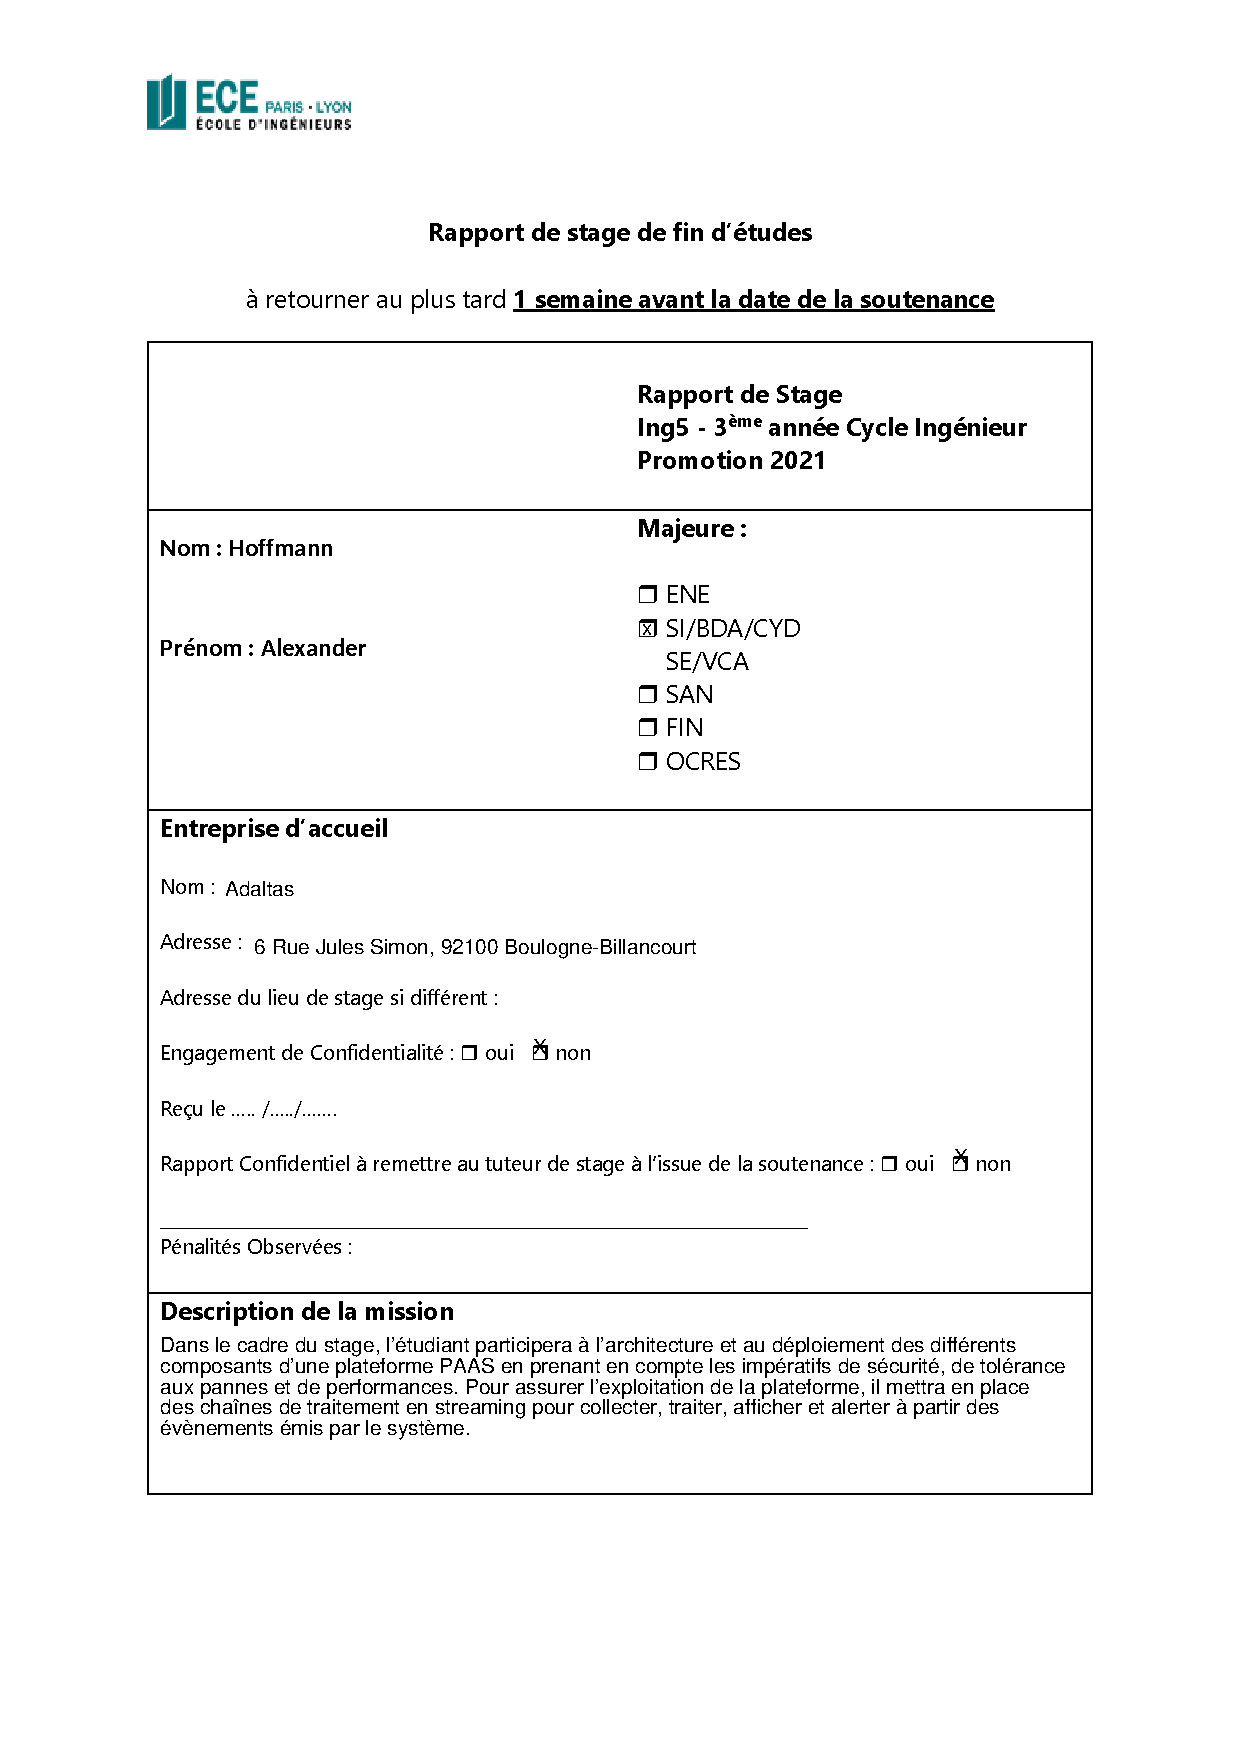
\includepdf[pages=-]{assets/pdf/title.pdf}

\maketitle

\newpage
\thispagestyle{empty}
\mbox{}
\newpage

\chapter*{Remerciements}

Les premiers pas dans le monde du travail se font rarement seul et sans aide ni soutien. Je souhaite remercier toutes les personnes ayant contribué à cette expérience professionnelle.\\

Je tiens tout d’abord à remercier toute l'équipe d'Adaltas pour son accueil, sa bienveillance et sa bonne humeur permanente. J'apprécie l'attention et la sollicitude qui m'ont été prodiguées par toute personne rencontrée.\\

Je voudrais ensuite exprimer ma sincère gratitude à David Worms, mon tuteur, pour la confiance qu’il a bien voulu m’accorder en acceptant de m'intégrer à Adaltas. Je le remercie pour sa grande disponibilité, sa patience, son soutien chaleureux et ses conseils avisés. Je tiens à lui exprimer ma profonde reconnaissance pour ses critiques constructives d’une rigueur absolue.\\

Mes remerciements s’adressent également à Prisca Borges pour son accueil, sa sympathie et ses conseils, ainsi qu'à Léo Schoukroun pour son encadrement et sa compréhension qu'il m'a accordé tout au long du stage.\\

En cette période inédite de crise sanitaire, j'ai eu la chance de pouvoir travailler avec une entreprise qui a su s'adapter aux difficultés posées par les mesures nécessaires à la protection de ses collaborateurs. Je suis reconnaissant d'avoir pu effectuer mon stage dans les meilleures conditions possibles.

\newpage
\thispagestyle{empty}
\mbox{}
\newpage

\chapter*{Résumé}

Ce rapport décrit les travaux effectués lors de mon stage de 6 mois chez Adaltas. J'ai travaillé sous la supervision de David Worms en tant que Infrastructure and Security Operations (InfraOps) Intern. En tant qu'ingénieur InfraOps, j'ai aidé à construire des systèmes automatisés, sécurisés, fiables et observables, ainsi que des processus permettant aux autres équipes d'Adaltas d'utiliser efficacement notre infrastructure pour lancer, exploiter et fournir des produits et services de grande qualité destinés aux clients et couvrant de multiples écosystèmes b2c, partenaires et vendeurs à travers le monde.\\

\noindent\textbf{Mots clés} : Big Data, DevOps, InfraOps.

\newpage
\thispagestyle{empty}
\mbox{}
\newpage

\begingroup
\hypersetup{linkcolor=black}
\listoffigures
\tableofcontents
\newpage
\endgroup

\chapter*{Introduction}
\addcontentsline{toc}{chapter}{Introduction}

Mon intérêt pour la data science et plus généralement pour l’informatique et les nouvelles technologies m’a amené à chercher un stage dans une société qui en a fait son cœur de métier. Au sein de l'équipe InfraOps d'Adaltas, j'ai trouvé une opportunité unique pour mettre à profit mes compétences en matière de développement et de conception. J'ai eu la chance de participer à la création de systèmes et d'outils d'infrastructure permettant la mise en production de nouveaux produits qui s'étendent sur des millions d'utilisateurs. Pour assurer l’exploitation de la plateforme, j'ai mis en place des chaînes de traitement en streaming pour collecter, traiter, afficher et alerter à partir des évènements émis par le système.\\

La thématique de ce stage s’inscrit dans un contexte d’appréhension et d'approfondissement du monde de l’entreprise. Dans ce rapport, nous présenterons dans un premier temps, le contexte du stage, c’est-à-dire que nous décrirons l’entreprise d’accueil, nous étudierons son secteur d’activité et sa culture. Dans un second temps, nous traduirons les différents aspects de ma mission et les attentes de l'entreprise. Finalement, nous verrons les compétences et qualités acquises à la suite de ce travail ainsi que ma valeur ajoutée pour Adaltas.

\chapter{Présentation de la structure d'accueil: Adaltas}

Fondée en 2004, Adaltas est une société d’expertise en High Tech construite à partir de deux idées :
\begin{itemize}
  \item[--] l’innovation comme facteur de différenciation décisif pour les entreprises;
  \item[--] la capacité à mobiliser les meilleurs talents comme condition de succès.\\
\end{itemize}

\begin{figure}[H]

\includegraphics[scale=0.4]{assets/img/logo-adaltas.png}
\centering
\caption{Logo d'Adaltas représentant un oiseau. Adaltas signifie "vers le haut".}
\label{fig:logo-adaltas}
\end{figure}

Adaltas aide ses clients à s’orienter dans le monde en perpétuelle évolution de l’Open Source, leur donnant les clés pour développer les meilleures solutions, qu’il s’agisse simplement d’écrire une application ou d’élaborer une plateforme de traitement stratégique à plus long terme. L'entreprise se définit comme un acteur du Big Data autour des technologies \gls{hadoop} et \gls{nosql}.

Les équipes apportent une expertise sur l’analyse et le traitement des données, leur gouvernance, le développement et la gestion opérationnelle. Les consultants adhèrent à la culture \gls{devops} et ils sont formés à la méthodologie \gls{sre}\footnote{\href{https://landing.google.com/sre/}{What is Site Reliability Engineering (SRE)?}}. Ils accompagnent leur client dans la mise en place d’infrastructures et d’applications résilientes, conscients des rapides innovations apportés par la communauté Open Source et de la nécessaire stabilité des systèmes.

L'expertise d'Adaltas dans le domaine Big Data a commencé dès 2009 par l'accompagnement de la société EDF et la collecte des données Linky dit compteurs intelligents. En 2012, la société a entrepris l’exploitation d'une plateforme commune à l'ensemble du groupe EDF avec la mise à disposition des composants de l’éco-système Hadoop. Le nombre de composants s'est élargi avec le temps ainsi que les services et les cas d’usage qui ont accosté sur la plateforme sécurisée et multi-tenante.

Depuis 2014, l’équipe s’est élargie en accueillant des talents majoritairement formés à l’ECE, école dans laquelle Adaltas est à l’initiative du programme Big Data. Adaltas donne également des cours au Data Science Tech Institute\footnote{\href{https://www.datasciencetech.institute/}{https://www.datasciencetech.institute/}} et à l’Université Paris-Sorbonne.

\section{Objectifs de l'entreprise}

L’acquisition d’un cluster à forte capacité répond à la volonté d’Adaltas de construire une offre de type \gls{paas} pour disposer et mettre à disposition des plateformes de Big Data et d’orchestration de conteneurs. Les plateformes sont utilisées pour l’acquisition de nouvelles compétences, l’évaluation de nouvelles technologies, l’utilisation d’outils \gls{devops} et la mise à disposition d’environnements de développement, de PoCs et d’exploitation. Elles hébergent des Data Lakes, des DataLabs, des traitements et des modèles de Data Science, des outils orientés \gls{devops} ou encore des services applicatifs. L’objectif est de porter cette offre à maturité.

Dans le cadre de ses cours et formations, Adaltas s'intéresse au domaine Big Data et Data Science. Les cours effectués au seins des différents établissements ont pour objectif de trouver des jeunes talents pour les faire monter en compétence. Ainsi, la société cherche à recruter et former ses futurs consultants le plus tôt possible afin qu'ils soient opérationnels dès la fin du stage de dernière année d'école.

\section{Une entreprise "open"}

Adaltas est une société “open”. Leur engagement se construit sur les fondations d’un code source ouvert, d’une collaboration ouverte, de standards ouverts et d’une formation ouverte.

Les entreprises et les gouvernements utilisent les technologies Open Source pour remplacer les solutions propriétaires. Initialement, ces acteurs ont été attirés par les réductions de coût et la promesse de s’affranchir de la dépendance d’un éditeur. L’Open Source est désormais central à la transformation digitale avec des avantages avérés dans la sécurité, la qualité, la personnalisation, la flexibilité, l’intéropérabilité, l’auditabilité et le soutien.

Adaltas maintient près de 50 dépôts Open Source sur \gls{github} et encourage chaque développeur et client à contribuer à ces projets.

\section{La culture d'Adaltas}

Adaltas préserve un esprit familial qui privilégie toujours une vision à long terme. L'entreprise a pour vocation d’assurer le développement de chacun de ses consultants dans le respect de leur identité et de leur autonomie en mettant à disposition toutes les ressources nécessaires. Chaque service ou fonctionnalité proposé est le fruit d’une collaboration où chacun contribue aux idées des autres. L'objectif principal est de créer les meilleures expériences possibles pour les clients.

Le respect de ces valeurs est l’une des clefs de la performance d'Adaltas, de son ancrage dans l’air du temps et dans la société qui l'entoure.

\section{RSE : Responsabilité Sociétale de l’Entreprise}

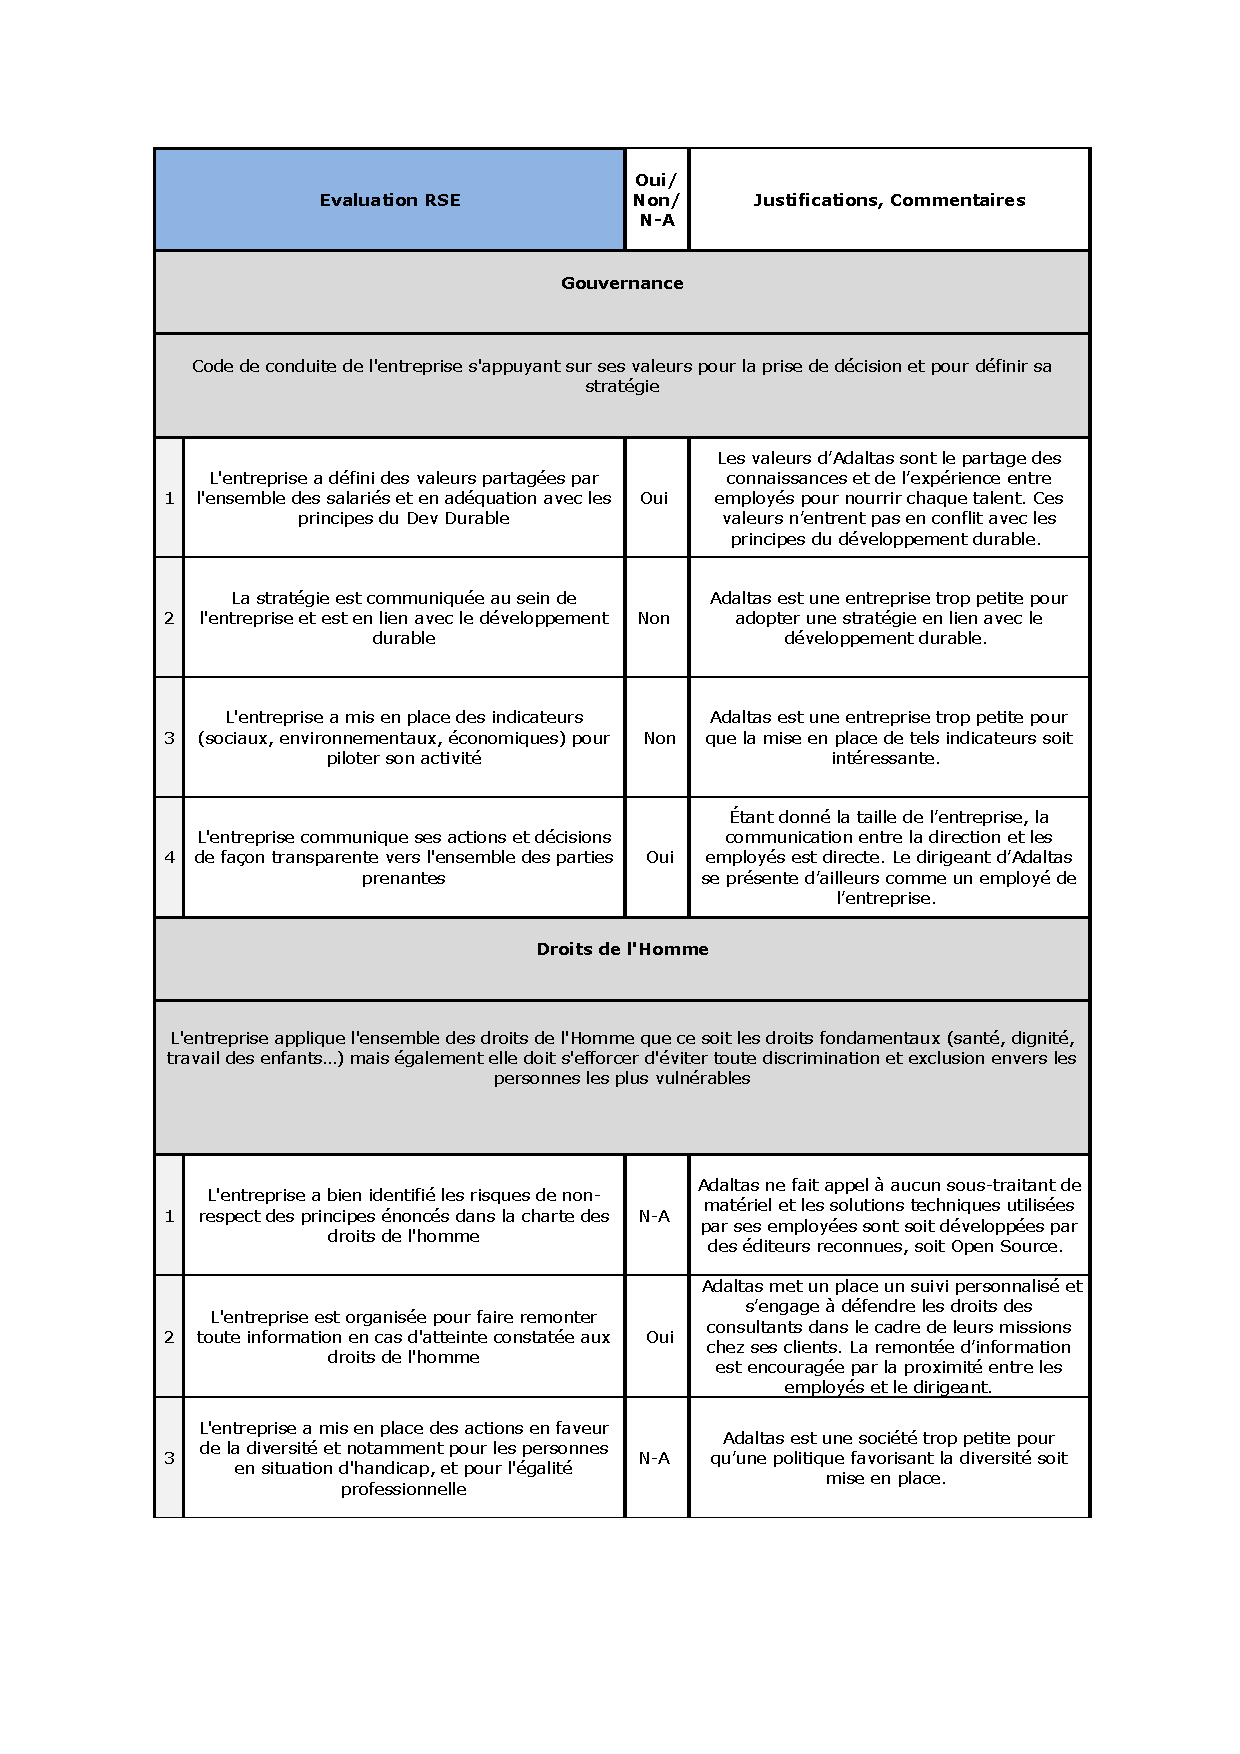
\includepdf[pages=-]{assets/pdf/rse.pdf}

\chapter{Présentation de la mission}

La mission principale de mon stage consistait à automatiser le déploiement d'un cluster Apache \gls{hadoop}.

\section{Cahier des charges}

Sur la base des différents objectifs présentés précédemment, un cahier des charges a été établi courant février 2021 par David Worms. Les activités précisées sont les suivantes : 

\begin{enumerate}
  \item Conception et mise en place d’architectures se basant sur des technologies open-source de l'écosystème Big Data ;
  \item Déploiement manuel d'un cluster \gls{hdp} ;
  \item Automatisation de l'installation, la configuration et le déploiement d'un cluster \gls{hdp} ;
  \item Rédaction d’articles pour partager les résultats des recherches.
\end{enumerate}

\section{Planning}

Le découpage temporel des missions proposées au début du stage est décrit sur la figure \ref{fig:planning}. Ce planning a été formulé en fonction de ma progression prévisionnelle de l'apprentissage des technologies Big Data. Lesdites technologies seront étudiées en détail ci-après.

\begin{figure}[h]
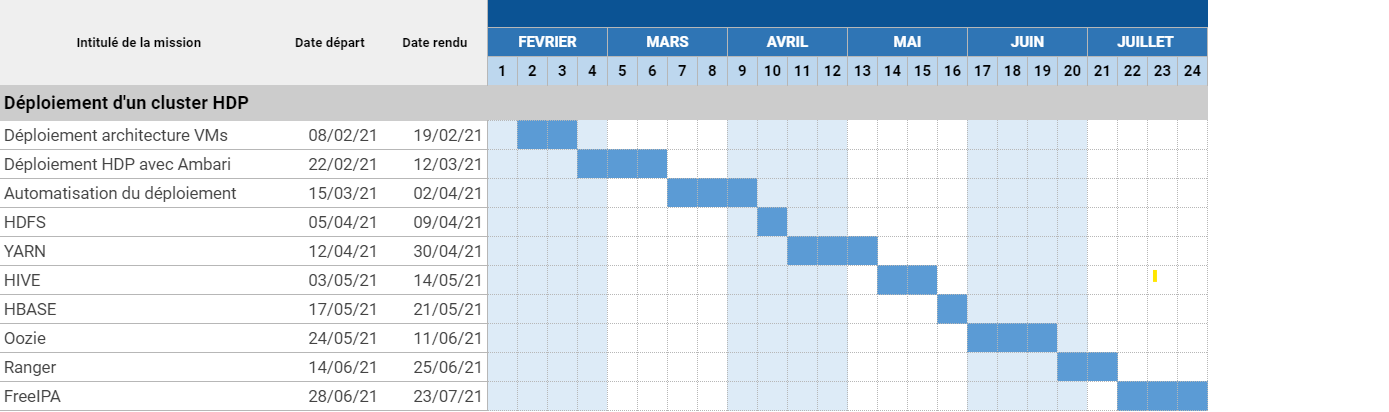
\includegraphics[scale=0.5]{assets/img/gantt.png}
\centering
\caption{Planning sous forme de diagramme de Gantt}
\label{fig:planning}
\end{figure}

\section{Environnement de travail}

La plus grande partie de mon stage s'est déroulée à distance. Quand j'étais sur les lieux de l'entreprise, j'ai eu l'opportunité de rencontrer et d'interagir de façon privilégiée avec les différentes collaborateurs. Les employés d’Adaltas ont des échanges quotidiens via le chat interne de l’entreprise (Keybase\footnote{\href{https://keybase.io/}{https://keybase.io/}}). Ainsi, j'ai pu solliciter l'expertise de chacun lorsque j'ai rencontré des difficultés.

Nous avions un meeting tous les deux jours pour faire un point sur l'avancée de nos missions. Cette réunion dure entre 15 et 20 minutes. Chaque membre de l'équipe prend la parole à tour de rôle et décrit au reste de l’équipe ce qu’il a fait la veille, les objectifs qui ont été atteints, ce qu’il prévoit de faire le reste de la journée avec les nouveaux objectifs, et les éventuels problèmes qu’il rencontre. De cette façon, il est facile de savoir qui peut lui venir en aide et comment, afin de résoudre ses problèmes et de lui permettre d’avancer de nouveau.

\section{Environnement de développement}

Pour remplir ma mission, Adaltas a mis à ma disposition un ordinateur à la pointe de la technologie. Il s'agit d'une machine de la marque Dell comportant les caratéristiques décrite dans la table \ref{tab:caractéristiques}.

\begin{table}[h]
\centering
\begin{tabular}{|l|l|}
\hline
\multicolumn{1}{|c|}{\textbf{Type de Hardware}} & \multicolumn{1}{c|}{\textbf{Caractéristiques techniques}}                          \\ \hline
Processeur                                      & Processeur Intel Core i7-9750H de 9e génération                                    \\ \hline
Disque                                          & Disque SSD hautes performances M.2 PCIE 40 de 1 To                                 \\ \hline
Mémoire                                         & 32 Go de mémoire, 2 x 16 Go, DDR4 à 2 666 MHz                                      \\ \hline
\end{tabular}
\caption{Caractéristiques techniques du matériel mis à disposition.}
\label{tab:caractéristiques}
\end{table}

Ces spécifications techniques sont nécessaires car les consultants sont amenés à créer des clusters Big Data avec plusieurs noeuds nécessitant une plus grande puissance de calcul. Au début de mon stage, j’ai dû installer \gls{arch} sur cet ordinateur. L’installation  habituellement assez périlleuse car il faut mettre en place un grand nombre de services manuellement (notamment les services réseaux et l’interface graphique). Pour faire face à cela, Adaltas a développé une solution nommée Nikita Arch\footnote{\href{https://github.com/adaltas/node-nikita-arch}{https://github.com/adaltas/node-nikita-arch}}, un logiciel de déploiement pour le système d'exploitation \gls{arch}. \gls{arch} est plus simple que Debian ou Ubuntu car \gls{pacman} ne touche pas à la configuration des paquets (ce que fait \gls{dpkg}). \gls{arch} est plus tolérant que Debian à propos des paquets "non-libres" tels que définis par \gls{gnu}. Il est optimisé pour x86\_64, et donc est plus rapide que Debian (i386). Les paquets d'\gls{arch} sont plus récents que les paquets Debian. En revanche Debian est largement plus stable, c'est pour ça qu'il est généralement utilisé pour les serveurs.

\chapter{Installation}

Ce chapitre couvre la description et l'installation de tous les outils nécessaires à ce projet. Tous les logiciels et paquets utilisés sont des logiciels Open Source et sont disponibles gratuitement.

\section{vim}

\begin{figure}[H]

\includegraphics[scale=0.1]{assets/img/logo-vim.png}
\centering
\caption{Logo de vim.}
\label{fig:logo-adaltas}
\end{figure}

Vim est un éditeur de texte directement inspiré de vi (un éditeur très répandu sur les systèmes d’exploitation de type Unix). Son nom signifie d’ailleurs Vi IMproved, que l’on peut traduire par « VI aMélioré ». A priori, Vim n'est pas un IDE mais un simple éditeur de texte. Néanmoins, l'ajout  d'extensions, ou la modification de son fichier de configuration en fait un environnement de développement optimal. L'avantage est qu'il n'est pas nécessaire de maîtriser plusieurs IDE, Vim suffit.

Etant donné que j'avais déjà quelques notions de Vim avant mon stage, j'ai été chargé de rédiger un tutoriel sur le site du cloud d'Adaltas. Cette introduction est destinée aux personnes n'ayant jamais utilisé Vim. Voici le \href{https://www.adaltas.cloud/en/docs/foundations/vim/}{lien} vers mon tutoriel.

\section{git}

\begin{figure}[H]

\includegraphics[scale=0.1]{assets/img/logo-git.png}
\centering
\caption{Logo de git.}
\label{fig:logo-adaltas}
\end{figure}

Git est un outil de contrôle de version similaire à \href{https://en.wikipedia.org/wiki/Concurrent_Versions_System}{CVS}, \href{https://subversion.apache.org/}{Subversion} et \href{https://www.mercurial-scm.org/}{Mercurial}. Cette famille d'outils s'appelle Système de Contrôle de Version (SCV) ou Gestion du Contrôle des Sources (GCS). Un contrôle de version permet de garder une trace des modifications apportées à un ou plusieurs fichiers au fil du temps afin de pouvoir accéder ultérieurement à une version spécifique. Voici quelques exemples : un développeur veut garder une trace de l'évolution de son code ; un ingénieur DevOps veut déclencher des tests sur les changements publiés et déployer de nouvelles versions à partir de points d'accès bien définis de l'historique du logiciel ; un développeur web a besoin de stocker chaque version d'une image ou d'une mise en page ; un ingénieur infrastructure veut stocker et garder une trace de ses procédures de déploiement et des changements de configuration ; un Data Scientist veut enregistrer toutes ses expériences et les évolutions des fonctionnalités. Chez Adaltas, la procédure d'installation des systèmes \gls{arch} utilisée sur la majorité de nos ordinateurs portables est stockée et partagée sur un dépôt public.

\section{VirtualBox}

\begin{figure}[H]

\includegraphics[scale=0.2]{assets/img/logo-virtualbox.png}
\centering
\caption{Logo de \gls{virtualbox}.}
\label{fig:logo-adaltas}
\end{figure}

Oracle VM \gls{virtualbox} est une application de virtualisation multiplateforme open-source. Le logiciel s'installe sur une machine physique basée sur Intel ou AMD, qu'elle fonctionne sous les systèmes d'exploitation (OS) Windows, Mac OS X, Linux ou Oracle Solaris. \gls{virtualbox} étend les capacités de la machine hôte afin d'y exécuter plusieurs OS, dans plusieurs machines virtuelles, en même temps. À titre d'exemple, il est possible d'exécuter Windows et Linux sur Mac, d'exécuter Windows Server 2016 sur un serveur Linux, d'exécuter Linux sur un PC Windows, et ainsi de suite, le tout aux côtés des applications existantes. Il est possible d'installer et d'exécuter autant de machines virtuelles que souhaité. Les seules limites pratiques sont l'espace disque et la mémoire. La capture d'écran de la figure \ref{fig:example-vbox} montre comment \gls{virtualbox}, installé sur un ordinateur Microsoft Windows 10, exécute Ubuntu 20.04 dans une machine virtuelle.

\begin{figure}[h]
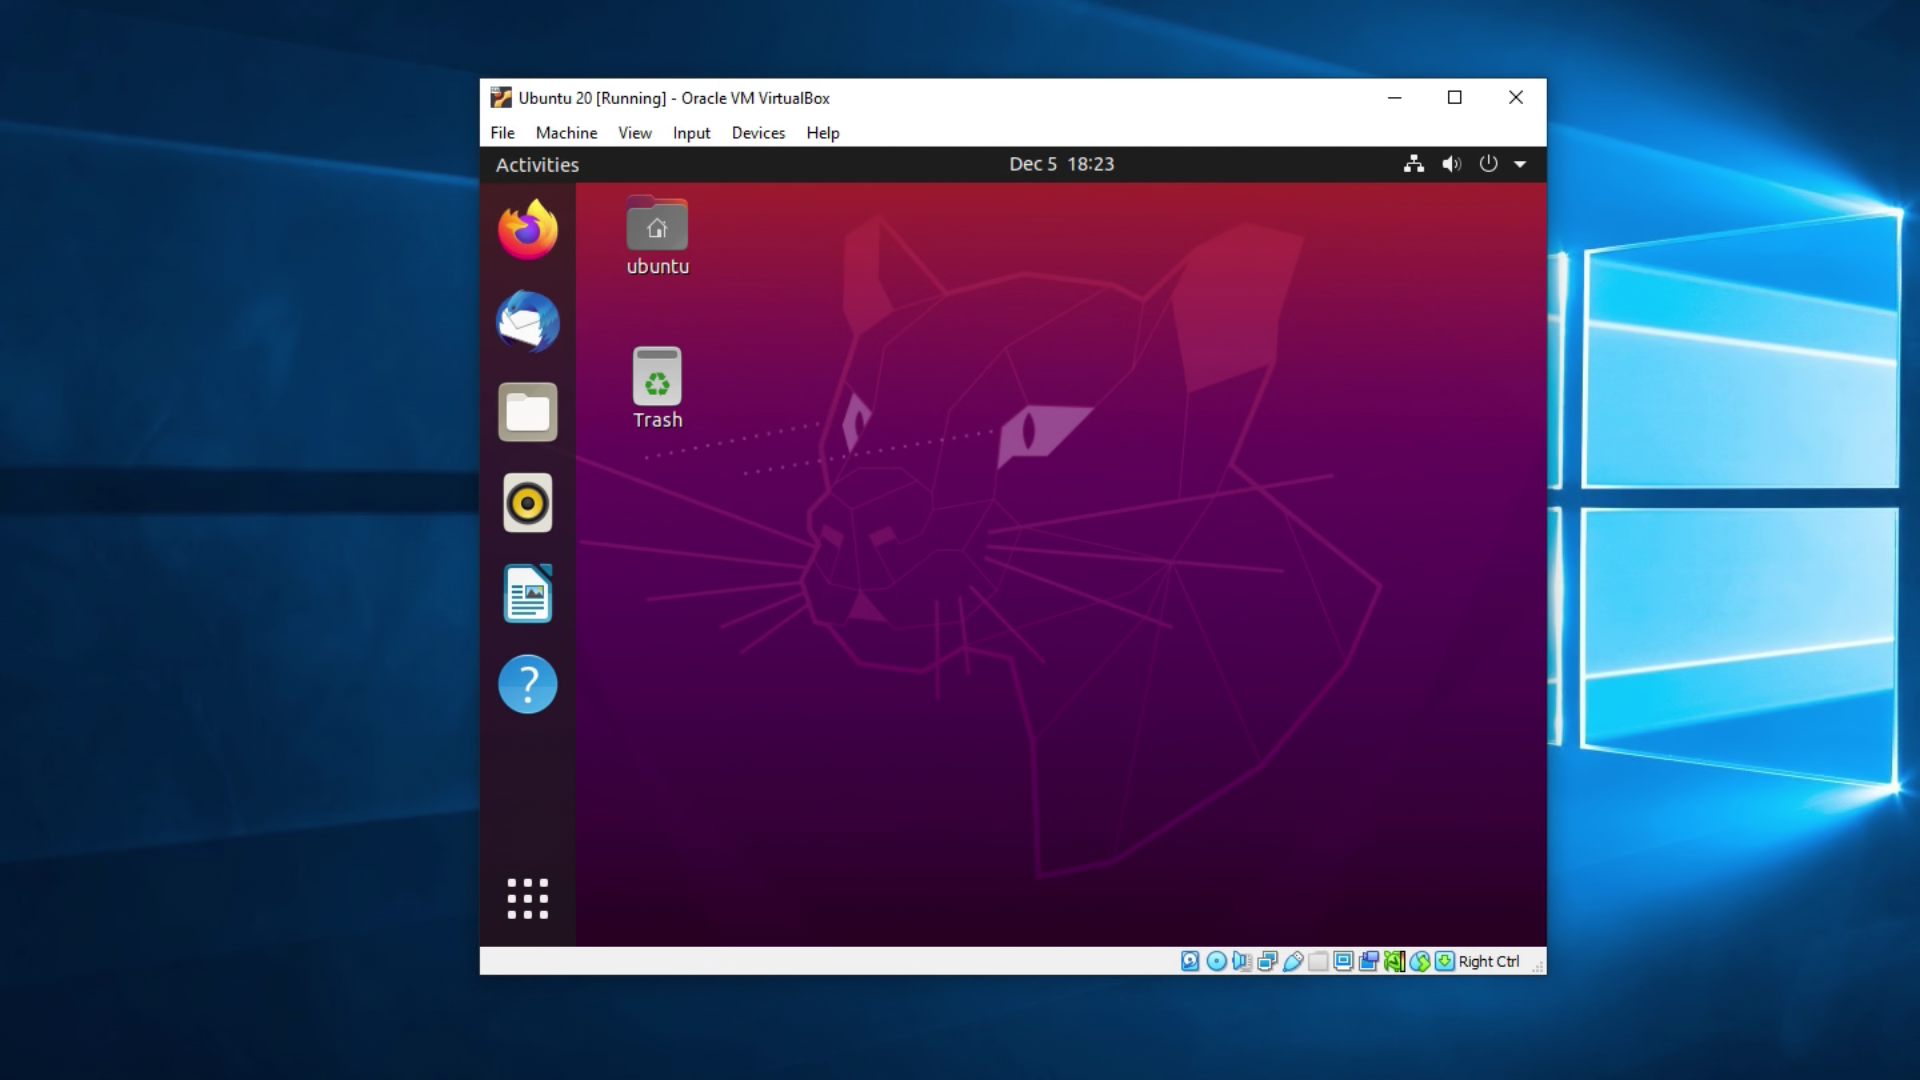
\includegraphics[scale=0.2]{assets/img/example-vbox.png}
\centering
\caption{Exemple d'utilisation de \gls{virtualbox}.}
\label{fig:example-vbox}
\end{figure}

L'utilisation de la virtualisation est un avantage majeur dans le domaine du Big Data étant donné que cela permet de mettre en place des environnements de développement et de test rapidement et de les supprimer sans complexité.

\section{Vagrant}

\begin{figure}[H]

\includegraphics[scale=0.5]{assets/img/logo-vagrant.png}
\centering
\caption{Logo de \gls{vagrant}.}
\label{fig:logo-adaltas}
\end{figure}

\gls{vagrant} est un outil permettant de créer et de gérer des environnements de machines virtuelles. \gls{vagrant} réduit le temps de configuration de l'environnement de développement et automatise le déploiement de plusieurs machines virtuelles. \gls{vagrant} fournit des environnements de travail faciles à configurer, reproductibles et portables afin d'optimiser la productivité et la flexibilité.

Pour créer et gérer des machines virtuelles, nous utilisons un \texttt{Vagrantfile}. La fonction principale du fichier \texttt{Vagrantfile} est de décrire le type de machine requis pour un projet, ainsi que la manière de configurer et de provisionner ces machines. \gls{vagrant} fonctionne avec un \texttt{Vagrantfile} par projet, et le fichier est sauvegardé dans le contrôle de version. Cela permet aux autres développeurs impliqués dans le projet de vérifier le code. Les fichiers \texttt{Vagrantfile} sont portables sur toutes les plateformes supportées par \gls{vagrant}. La syntaxe des \texttt{Vagrantfile} est Ruby, mais la connaissance du langage de programmation Ruby n'est pas nécessaire pour apporter des modifications au fichier, puisqu'il s'agit principalement de simples affectations de variables. La figure \ref{fig:example-vagrantfile} montre un exemple de fichier \texttt{Vagrantfile} utilisé pour un cluster de développement.

\begin{figure}[h]
\begin{verbatim}
box = "centos/7"

Vagrant.configure("2") do |config|
  config.vm.synced_folder ".", "/vagrant", disabled: true
  config.ssh.insert_key = false
  config.vm.box_check_update = false
  config.vm.define :master01 do |node|
    node.vm.box = box
    node.vm.network :private_network, ip: "10.10.10.11"
    node.vm.provider "virtualbox" do |d|
      d.memory = 8192
    end
    node.vm.hostname = "master01.nikita.local"
  end
  config.vm.define :worker01 do |node|
    node.vm.box = box
    node.vm.network :private_network, ip: "10.10.10.16"
    node.vm.provider "virtualbox" do |d|
      d.customize ["modifyvm", :id, "--memory", 2048]
      d.customize ["modifyvm", :id, "--cpus", 2]
      d.customize ["modifyvm", :id, "--ioapic", "on"]
    end
    node.vm.hostname = "worker01.nikita.local"
  end
end
\end{verbatim}
\centering
\caption{Exemple de fichier \texttt{Vagrantfile}.}
\label{fig:example-vagrantfile}
\end{figure}

Les Box sont le format de paquetage des environnements \gls{vagrant}. Une Box peut être utilisée par n'importe qui, sur n'importe quelle plate-forme prise en charge par \gls{vagrant}, pour créer un environnement de travail. Le moyen le plus simple d'utiliser une Box est d'en ajouter une à partir du catalogue accessible au public. Pour la création du cluster, j'ai utilisé la Box \gls{centos} version 7 car c'est l'une des distributions Linux la plus stable et rapide à configurer.

\section{Ansible}

\begin{figure}[h]

\includegraphics[scale=0.07]{assets/img/logo-ansible.png}
\centering
\caption{Logo de \gls{ansible}.}
\label{fig:logo-ansible}
\end{figure}

\gls{ansible} est un logiciel d'automatisation informatique qui automatise le provisionnement des clouds, la gestion de la configuration, le déploiement des applications, l'orchestration intra-service et de nombreux autres besoins informatiques. \gls{ansible} fonctionne en se connectant aux nœuds et en leur envoyant des scripts, appelés "modules Ansible". Ces programmes sont écrits pour être des modèles de ressources de l'état souhaité du système. Ansible exécute ensuite ces modules (via SSH par défaut), et les supprime une fois terminés.

Par défaut, Ansible représente les machines gérées en utilisant un fichier INI qui place toutes les machines dans des groupes définis. Le fichier que j'ai utilisé pour le déploiement du cluster est décrit sur la figure \ref{fig:example-ansible-inventory}.

\begin{figure}[h]
\begin{verbatim}
[cloudera_manager]
master01.nikita.local

[cluster_master_nodes]
master01.nikita.local host_template=Master1

[cluster_worker_nodes]
worker01.nikita.local

[cluster_worker_nodes:vars]
host_template=Workers

[cluster:children]
cluster_master_nodes
cluster_worker_nodes

[db_server]
master01.nikita.local

[deployment:children]
cluster
db_server

[deployment:vars]
# Ansible will defer to the running SSH Agent for relevant keys
# Set the following to hardcode the SSH private key for the instances
# ansible_ssh_private_key_file=~/.ssh/mykey.pem  
ansible_user=vagrant
\end{verbatim}
\centering
\caption{Exemple de fichier \texttt{inventory.ini}.}
\label{fig:example-ansible-inventory}
\end{figure}

\section{Ambari}

\begin{figure}[H]

\includegraphics[scale=0.2]{assets/img/logo-ambari.png}
\centering
\caption{Logo de \gls{ambari}.}
\label{fig:logo-ambari}
\end{figure}

Le projet Apache \gls{ambari} vise à simplifier la gestion d'\gls{hadoop} en développant un logiciel pour le provisionnement, la gestion et la surveillance de clusters Apache \gls{hadoop}. Ambari fournit une interface web de gestion intuitive et facile à utiliser, soutenue par ses API RESTful. \gls{ambari} permet aux administrateurs système de provisionner un cluster \gls{hadoop} grâce à un assistant qui guide l'utilisateur étape par étape pour l'installation des services sur tous les hôtes. De plus, le logiciel fournit une gestion centrale pour le démarrage, l'arrêt et la reconfiguration des services sur l'ensemble du cluster. Enfin, \gls{ambari} fournit un tableau de bord pour surveiller la santé et l'état du cluster.

\section{Hadoop}

\begin{figure}[H]

\includegraphics[scale=0.2]{assets/img/logo-hadoop.png}
\centering
\caption{Logo de \gls{hadoop}.}
\label{fig:logo-hadoop}
\end{figure}

Apache \gls{hadoop} est un logiciel open-source pour le stockage et le traitement à grande échelle d'ensembles de données sur des clusters. Il est composé des modules suivants :
\begin{itemize}
  \item[--] Hadoop Common : contient des bibliothèques et des utilitaires nécessaires aux autres modules Hadoop.
  \item[--] Hadoop YARN : une plateforme de gestion des ressources chargée de gérer les ressources de calcul dans les clusters et de les utiliser pour la programmation des applications des utilisateurs.
  \item[--] Hadoop MapReduce : un modèle de programmation pour le traitement de données à grande échelle.
  \item[--] Hadoop Distributed File System (HDFS) : un système de fichiers distribué qui stocke les données sur des machines de base, offrant une bande passante globale très élevée dans le cluster.\\
\end{itemize}

\subsection{Stack Hadoop}

\gls{hadoop} et ses différents composants s'assemblent pour garantir un modèle de stockage et de gestion des Big Data tolérant aux pannes, durable et hautement efficace. Un cluster Big Data peut être décomposé en plusieurs noeuds :

\begin{description}
  \item[Namenode] Namenode est le nœud qui stocke les métadonnées du système de fichiers, c'est-à-dire quel fichier correspond à quel emplacement de bloc et quels blocs sont stockés sur quel datanode. Le namenode maintient deux tables en mémoire, l'une qui mappe les blocs aux datanodes (un bloc mappe à 3 datanodes pour une valeur de réplication de 3) et une mappe de numéro de bloc à datanode. Chaque fois qu'un nœud de données signale une corruption de disque d'un bloc particulier, la première table est mise à jour et chaque fois qu'un nœud de données est détecté comme étant mort (à cause d'une panne de nœud/réseau), les deux tables sont mises à jour.
  \item[Secondary Namenode] Le noeud secondaire se connecte régulièrement au noeud primaire et récupère des métadonnées du système de fichiers dans le stockage local ou distant.
  \item[Datanode] Le Datanode est l'endroit où se trouvent les données.
\end{description}
Associés à ces différents types de noeuds, il existe des gestionnaires
\begin{description}
  \item[Node Manager] Il s'agit d'un démon yarn qui fonctionne sur des nœuds individuels et reçoit des informations sur les conteneurs de ressources de leurs Datanodes individuels via des démons. Les différentes ressources telles que la mémoire, le temps processeur, la bande passante du réseau, etc. sont regroupées dans une unité appelée conteneur de ressources. Le Node Manager assure à son tour la tolérance aux pannes sur les Datanodes pour tous les travaux MapReduce.
  \item[Resource Manager] Il s'agit d'un démon yarn qui gère l'allocation des ressources aux différents jobs et qui comprend un planificateur qui s'occupe de la programmation des jobs.
\end{description}

\chapter{Déploiement d’un cluster Hadoop}

Cette section décrit la méthodologie permettant l'installation et la configuration de l'écosystème Hadoop dans un cluster multinode. J'ai mis en place une architecture composée de deux nœuds, un master et un worker. Pour ce projet, j'ai utilisé Ambari 2.7.3 et HDP-3.1.4. Les fichiers sources sont disponibles sur le cloud d'Adaltas à l'adresse suivante : \href{https://repos.adaltas.cloud/}{https://repos.adaltas.cloud/}.

\section{Déploiement de l'architecture}

Ce projet a été lancé avec un cluster multinode. Pour cela, il est nécessaire de déployer deux machines virtuelles \gls{centos} 7 et de les configurer de telle sorte à ce qu'elles puissent accueillir les différents services du cluster. Le déploiement de ces vms est effectué en quelques commandes grâce à \gls{vagrant}. Le \texttt{Vagrantfile} utilisé est décrit dans la figure \ref{fig:example-vagrantfile}. Le cluster est constitué des noeuds \texttt{master01} et \texttt{worker01} dont les caractéristiques sont décrites respectivement dans les figures \ref{tab:caractéristiques-cluster-master01} et \ref{tab:caractéristiques-cluster-worker01}.

\begin{table}[h]
\centering
\begin{tabular}{|l|l|}
\hline
\multicolumn{1}{|c|}{\textbf{Intitulé}} & \multicolumn{1}{c|}{\textbf{Valeur}}         \\ \hline
FQDN                                      & master01.nikita.local                      \\ \hline
Adresse IP                                & 10.10.10.11                                \\ \hline
Mémoire                                   & 8192 MB                                    \\ \hline
\end{tabular}
\caption{Caractéristiques du noeud \texttt{master01}.}
\label{tab:caractéristiques-cluster-master01}
\end{table}

\begin{table}[h]
\centering
\begin{tabular}{|l|l|}
\hline
\multicolumn{1}{|c|}{\textbf{Intitulé}} & \multicolumn{1}{c|}{\textbf{Valeur}}         \\ \hline
FQDN                                      & worker01.nikita.local                      \\ \hline
Adresse IP                                & 10.10.10.16                                \\ \hline
Mémoire                                   & 2048 MB                                    \\ \hline
\end{tabular}
\caption{Caractéristiques du noeud \texttt{worker01}.}
\label{tab:caractéristiques-cluster-worker01}
\end{table}

Une fois ces machines définies dans le \texttt{Vagrantfile}, il suffit de taper la commande suivante pour démarrer les noeuds :

\begin{verbatim}
$ vagrant up
\end{verbatim}

Nous avons maintenant un cluster avec deux machines virtuelles \gls{centos} 7 vierges qui seront utilisées pour installer les différents services \gls{hadoop}.

\section{Installation manuelle}

\subsection{Prérequis}

Avant de pouvoir installer les composants, il est nécessaire d'effectuerquelques prérequis afin d'assurer le bon fonctionnement du cluster.

\subsubsection{Configuration de SSH sans mot de passe}

Pour qu'\gls{ambari} Server installe automatiquement les Agents \gls{ambari} sur tous les hôtes du cluster, il faut configurer des connexions SSH sans mot de passe entre l'hôte \gls{ambari} Server et tous les autres hôtes du cluster. L'hôte \gls{ambari} Server utilise l'authentification par clé publique SSH pour accéder à distance et installer l'agent \gls{ambari}. Autrement, il est possible d'installer manuellement un Agent \gls{ambari} sur chaque hôte du cluster. Dans ce cas, il n'est pas nécessaire de générer et de distribuer des clés SSH. La première méthode est recommandée car elle permet de définir les connexions entre les noeuds avant la mise en place d'\gls{ambari}.

\subsubsection{Création des comptes utilisateurs de service}

Chaque service nécessite un compte utilisateur de service. L'assistant d'installation d'\gls{ambari} crée de nouveaux comptes d'utilisateur et utilise ces derniers lors de la configuration des services \gls{hadoop}. La création de comptes d'utilisateur de service s'applique aux comptes d'utilisateur de service sur le système d'exploitation local et aux comptes LDAP/AD. Par exemple, pour le service Hive, il faut créer un compte utilisateur \texttt{hive} sur tous les noeuds du cluster. Cette opération permet aux services Hive Metastore, HiveServer2 de fonctionner.

\subsubsection{Configuration du DNS}

Tous les hôtes du cluster doivent être configurés convenablement au niveau de la résolution DNS direct et inverse. Pour cela, il suffit de modifier le fichier \texttt{/etc/hosts} sur chaque hôte afin d'y ajouter l'adresse IP et le nom de domaine complet (FQDN) de chaque machine. \gls{hadoop} s'appuie fortement sur le DNS et effectue de nombreuses résolutions DNS en fonctionnement normal. Dans notre exemple, chaque VM contient les entrées suivantes dans le fichier \texttt{/etc/hosts} :

\begin{verbatim}
127.0.0.1   localhost
::1         localhost
10.10.10.11 master01.nikita.local
10.10.10.16 worker01.nikita.local
\end{verbatim}

\subsubsection{Configuration des connecteurs de base de données}

Les services tels que Druid, Hive, Ranger et Oozie nécessitent une base de données opérationnelle. Pour qu'\gls{ambari} puisse se connecter à une base de données, il faut télécharger les pilotes de base de données et les connecteurs nécessaires avant d'installer le composant. Il est possible d'utiliser les bases de données MySQL, Oracle, PostgreSQL ou Amazon RDS. Dans notre cas, nous utilisons MySQL que nous installons sur un noeud qui sera utilisé comme serveur BDD.

\subsection{Installation depuis un dossier dans le cloud}

Les fichiers sources permettant l'installation de \gls{hdp} et d'\gls{ambari} sont hébergés sur un dossier dans le cloud d'Adaltas accessible à l'adresse suivante : \href{https://repos.adaltas.cloud/}{https://repos.adaltas.cloud/}. Cela permet de bénéficier d'une plus grande gouvernance et de meilleures performances d'installation. Ensuite, il suffit de modifier le fichier \texttt{ambari.repo} et de remplacer l'URL de base \gls{ambari} \texttt{baseurl} obtenue lors de la configuration.

A présent, il s'agit de télécharger \gls{ambari} Server sur le noeud principal, c'est-à-dire \texttt{master01}. Avant de démarrer le serveur Ambari, il faut le configurer. L'installation configure la connexion à la base de données, installe le JDK et permet de personnaliser le compte utilisateur sous lequel le démon Ambari Server s'exécutera. La commande \texttt{ambari-server setup} gère le processus d'installation.

\subsection{Configuration et déploiement d'un cluster}

Pour installer, configurer et déployer un cluster \gls{hdp}, il faut encore effectuer plusieurs opérations sur l'invité de commande du noeud principal ainsi que sur l'interface web d'\gls{ambari}.

\subsubsection{Démarrage du serveur Ambari}

Exécuter la commande suivante sur l'hôte du serveur \gls{ambari} :

\begin{verbatim}
ambari-server start
\end{verbatim}

\subsubsection{Connexion à l'interface Ambari}

Pour se connecter à Ambari Web, il suffit d'ouvrir le navigateur web à l'adresse \texttt{\href{http://master01.nikita.local/8080}{http://master01.nikita.local/8080}} et de se connecter au serveur en utilisant le nom d'utilisateur/mot de passe par défaut : admin/admin. Pour un nouveau cluster, l'assistant d'installation de cluster affiche une page de bienvenue comme le montre la figure \ref{fig:wizard-ambari}.

\begin{figure}[h]
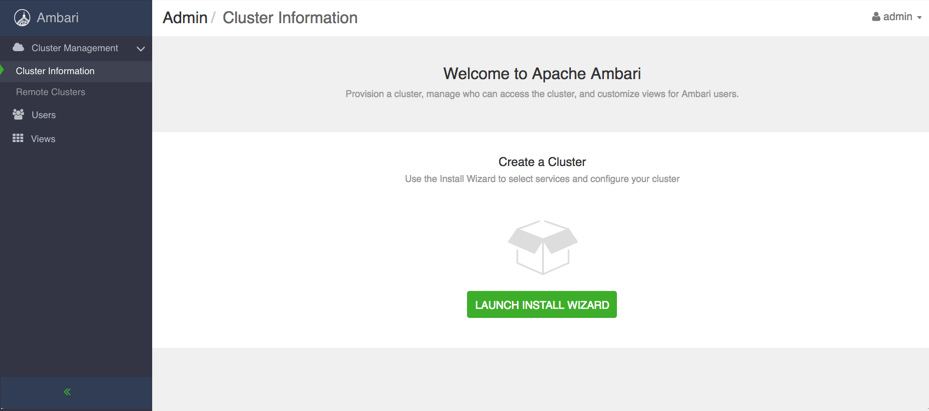
\includegraphics[scale=0.6]{assets/img/ambari-wizard.png}
\centering
\caption{Ecran de bienvenue de l'assistant d'installation \gls{ambari}.}
\label{fig:wizard-ambari}
\end{figure}

A présent, il s'agit de lancer l'assistant d'installation de cluster d'\gls{ambari} durant lequel il faudra effectuer les étapes suivantes :

\begin{enumerate}
\item Attribuer un nom au cluster
\item Sélectionner la version de \gls{hdp}
\item Fournir le FQDN de chacun des noeuds
\item Confirmer qu'\gls{ambari} a localisé tous les hôtes pour s'assurer qu'ils ont les les paquets et les processus requis
\item Sélectionner les services souhaités au sein du cluster
\item Assigner les noeuds "master"
\item Assigner les noeuds "esclaves"
\item Configurer les services
\item Confirmer la configuration
\end{enumerate}

Fort de toutes les étapes que nous venons d'effectuer, nous avons déployé un cluster \gls{hdp} localement. Cela étant, cette méthodologie n'est pas viable si l'on venait à déployer une centaine de clusters sur plusieurs infrastructures indépendantes. Ainsi, il nous faut trouver une solution qui permettrait d'automatiser toutes les étapes redondantes telles que l'installation de la base de données ou encore la configuration du DNS.

\section{Automatisation de l'installation et du déploiement}

La méthode d'installation décrite dans la section précédente n'est pas viable car elle est chronophage et répétitive. Afin de valoriser le temps passé à mettre en place le cluster, il s'agira d'automatiser l'installation et le déploiement du cluster.

\subsection{Automatisation avec Ansible}

\gls{ansible} permet la configuration, le déploiement, le provisionnement, et l'orchestration de clusters multi-nœuds. Pour cela, il existe un concept nommé \textbf{playbook}. Les playbooks enregistrent et exécutent les fonctions de configuration, de déploiement et d'orchestration d'Ansible. Ils peuvent décrire une configuration à appliquer pour les systèmes, ou un ensemble d'étapes d'un processus informatique général. Les playbooks sont conçus pour être lisibles par l'homme et sont développés dans un langage texte de base. Pour l'automatisation du déploiement, j'ai créé un playbook Ansible, inspiré de celui mis à disposition par Hortonworks\footnote{\href{https://github.com/hortonworks/ansible-hortonworks}{https://github.com/hortonworks/ansible-hortonworks}}, capable de construire un cluster \gls{hdp} en utilisant Ambari Blueprints. Les Blueprints d'Ambari sont une définition déclarative d'un cluster. Avec un Blueprint, il est possible de définir le Stack Hadoop, la disposition des composants et les configurations pour matérialiser une instance de cluster Hadoop (via une \gls{api}) sans avoir à utiliser l'assistant d'installation de cluster Ambari. Ainsi, le playbook se charge des étapes suivantes :

\begin{enumerate}
\item Préparation des noeuds (prérequis)
\item Installation d'\gls{ambari}
\item Configuration d'\gls{ambari}
\item Déploiement du Blueprint
\item Post-installation (tests fonctionnels)
\end{enumerate}

Avec cette méthodologie, nous arrivons au même résultat qu'avec l'installation manuelle. Il est possible de modifier quelques fichiers de configuration et ainsi de déployer n'importe quel cluster sur n'importe quelle infrastructure.

\section{Services Hadoop}

Dans cette section, nous décrivons les services Hadoop installés sur le cluster, indépendamment de la méthodologie utilisée.

\subsection{HDFS}

Hadoop Distributed File System (HDFS) est un système de fichiers distribués. HDFS est hautement tolérant aux pannes. Il fournit un accès haut débit aux données et convient à des applications qui ont de grands ensembles de données. HDFS assouplit quelques exigences POSIX pour permettre un accès en continu aux données du système de fichiers.

\subsection{YARN}

YARN est un système d'exploitation distribué à grande échelle pour les applications big data. Cette technologie est conçue pour la gestion de clusters. YARN est capable de découpler les capacités de gestion et d'ordonnancement des ressources de MapReduce du composant de traitement des données.

\subsection{HBase}

HBase est un système de gestion de base de données non relationnelle, open-source, distribuée, versionnée, qui fonctionne au-dessus du système de fichiers distribués Hadoop (HDFS). HBase offre un moyen tolérant aux pannes de stocker des ensembles de données, ce qui est courant dans de nombreux cas d'utilisation du Big Data. Il est bien adapté au traitement des données en temps réel ou à l'accès aléatoire en lecture/écriture à de grands volumes de données.

\subsection{Hive}

Hive est utilisé comme substitut de SQL pour le système de fichiers Hadoop, ce qui permet aux utilisateurs connaissant SQL d'interroger facilement des données à partir de ce système au lieu de devoir apprendre Map-Reduce. Le logiciel facilite la lecture, l'écriture et la gestion de grands ensembles de données au sein d'un stockage distribué.

\subsection{Spark}

Apache Spark est un moteur d'analyse unifié pour le traitement des données à grande échelle. Il fournit des API de haut niveau en Java, Scala, Python et R, ainsi qu'un moteur optimisé qui prend en charge les graphes d'exécution généraux. Il prend également en charge un riche ensemble d'outils de plus haut niveau, notamment Spark SQL pour le traitement des données SQL et structurées, MLlib pour l'apprentissage automatique, GraphX pour le traitement des graphes et Structured Streaming pour le calcul incrémental et le traitement en continu.

\subsection{Oozie}

Apache Oozie est un logiciel utilisé pour planifier les travaux Apache Hadoop. Oozie combine plusieurs travaux de manière séquentielle en une seule unité logique de travail. Il est intégré au Stack Hadoop, avec YARN comme centre architectural, et prend en charge les travaux Hadoop pour Apache MapReduce, Apache Pig, Apache Hive et Apache Sqoop. Oozie peut également planifier des tâches spécifiques à un système, comme des programmes Java ou des scripts shell.

\subsection{Ranger}

Apache Ranger est un logiciel permettant de mettre en place la sécurité d'un cluster Hadoop. Il fournit une plateforme centralisée pour définir, administrer et gérer les politiques de sécurité de manière cohérente à travers les services Hadoop.

\chapter*{Conclusion et perspectives}
\addcontentsline{toc}{chapter}{Bilan et perspectives}

Fort des éléments énoncés précédemment, ce stage technique effectué au sein de l’entreprise Adaltas constitue une expérience des plus enrichissantes étant donné la complexité technique des missions auxquelles j'ai pu prétendre participer. Outre l’aventure humaine enrichissante que j’eus la chance et le privilège de vivre, ce stage m’apprit le sens de la rigueur, du professionnalisme, ainsi que l’importance du temps et de son agencement. Grâce à cette expérience, j’ai acquis des nouvelles compétences qui me seront utiles pour mes futurs projets. De plus, les différentes missions effectuées m’ont permis d’accroître ma volonté de savoir et de connaissance, notamment dans le domaine du Big Data.\\

La réalisation des travaux décrits dans ce rapport m'a permis d'acquérir de nouvelles compétences en matière de développement, de gestion et de déploiement d'un cluster Big Data. J'ai appris à construire des systèmes faciles à utiliser, automatisés, sécurisés et fiables.\\

En terme de compétences techniques nouvellement acquises, nous pouvons énoncer :

\begin{itemize}
\item [--] Configuration et utilisation de systèmes et outils d'infrastructure
\item [--] Déploiement de systèmes évolutifs avec une infrastructure de production
\item [--] Automatisation du déploiement et provisionnement de clusters Big Data
\end{itemize}

\clearpage

\printglossaries

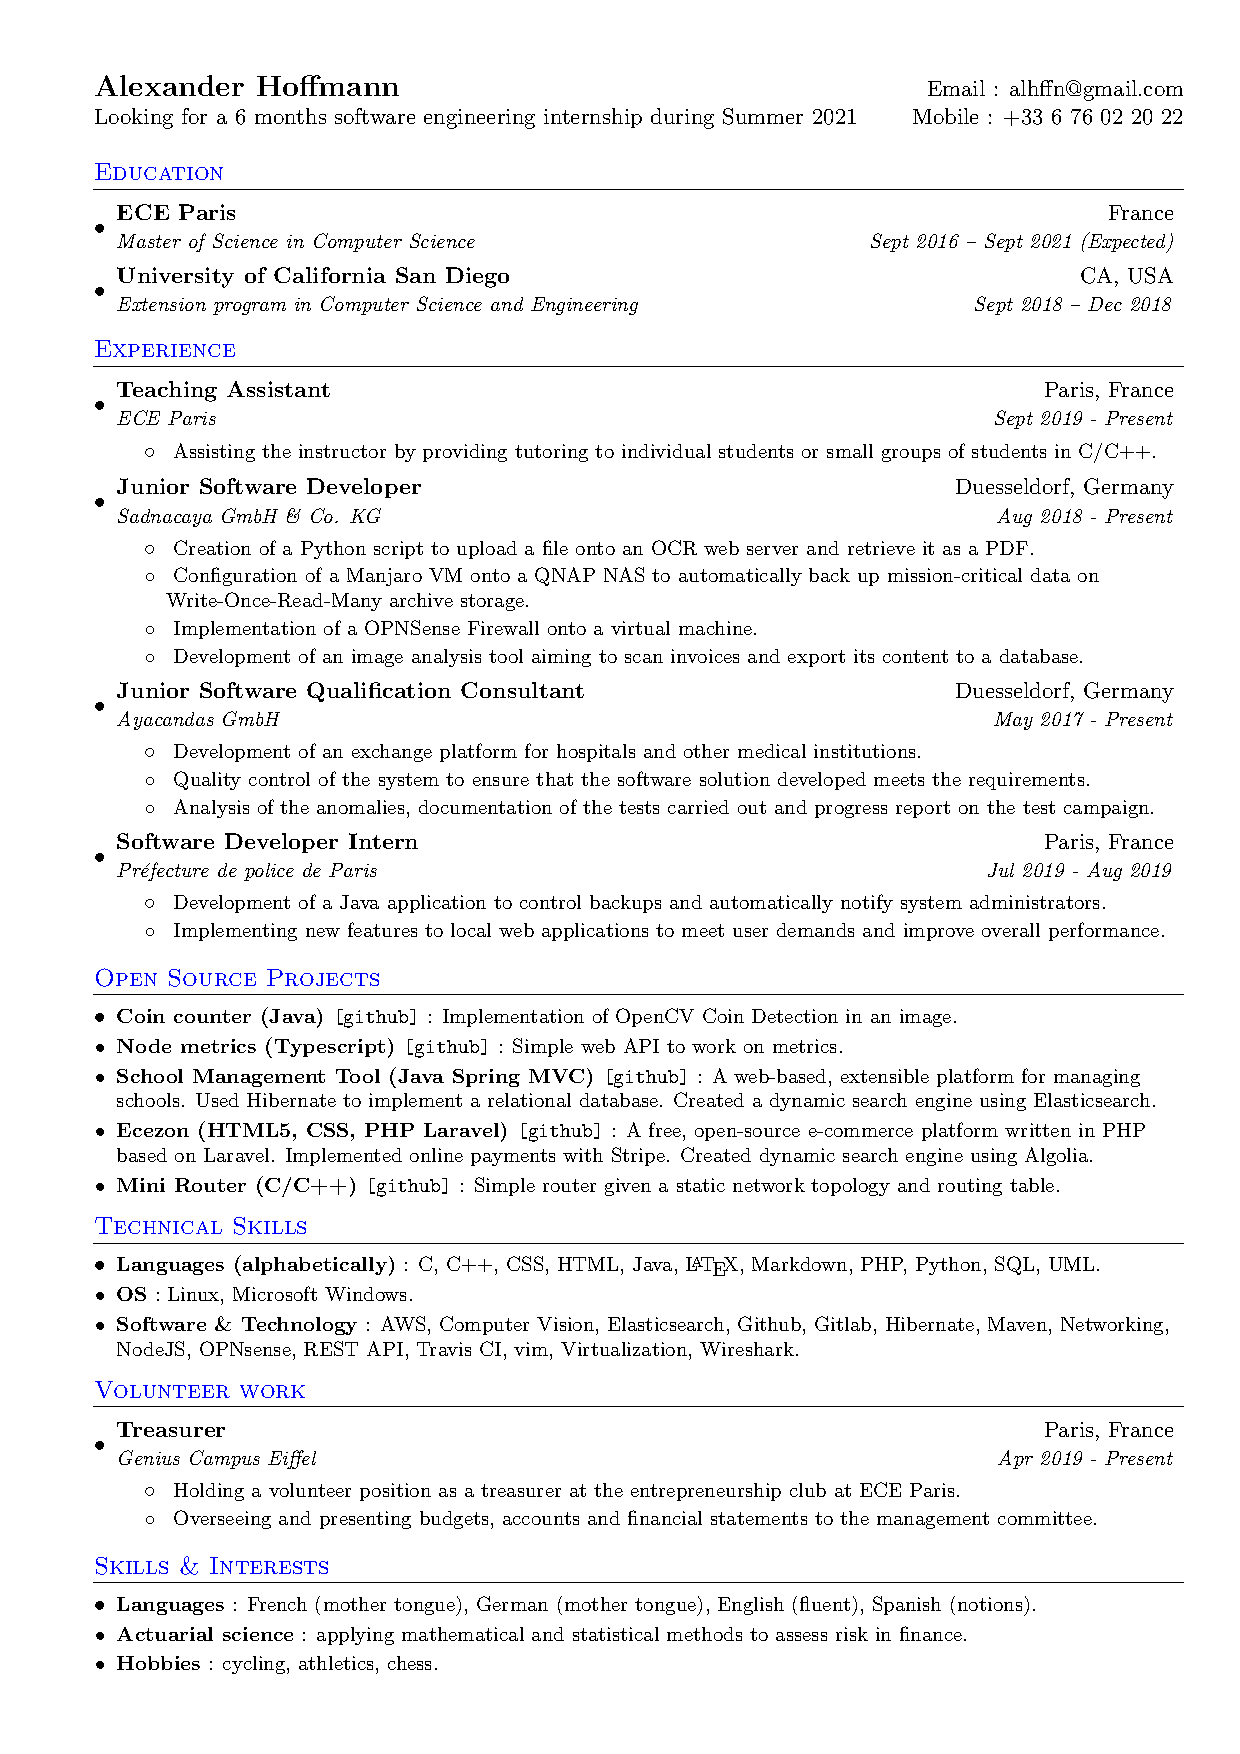
\includepdf[pages=-]{assets/pdf/resume-old.pdf}
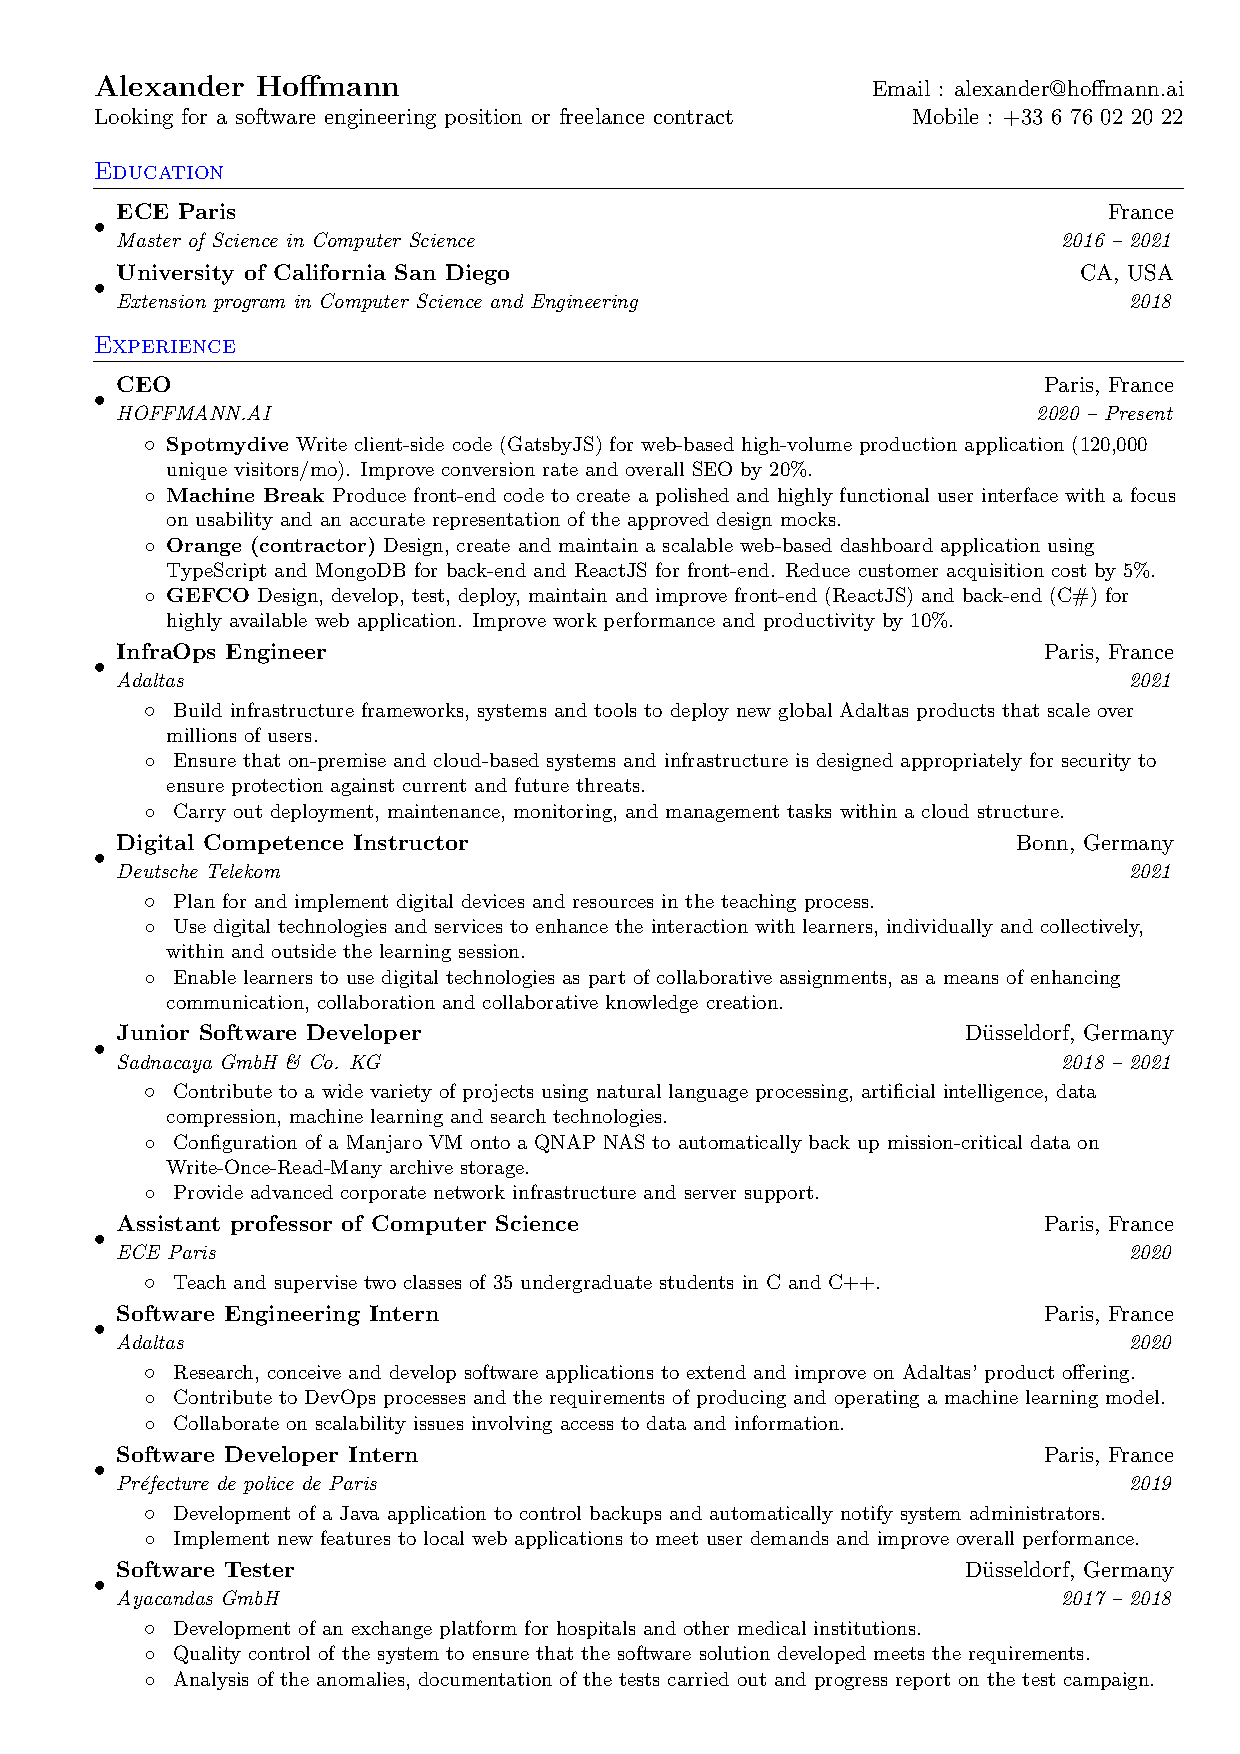
\includepdf[pages=-]{assets/pdf/resume-new.pdf}
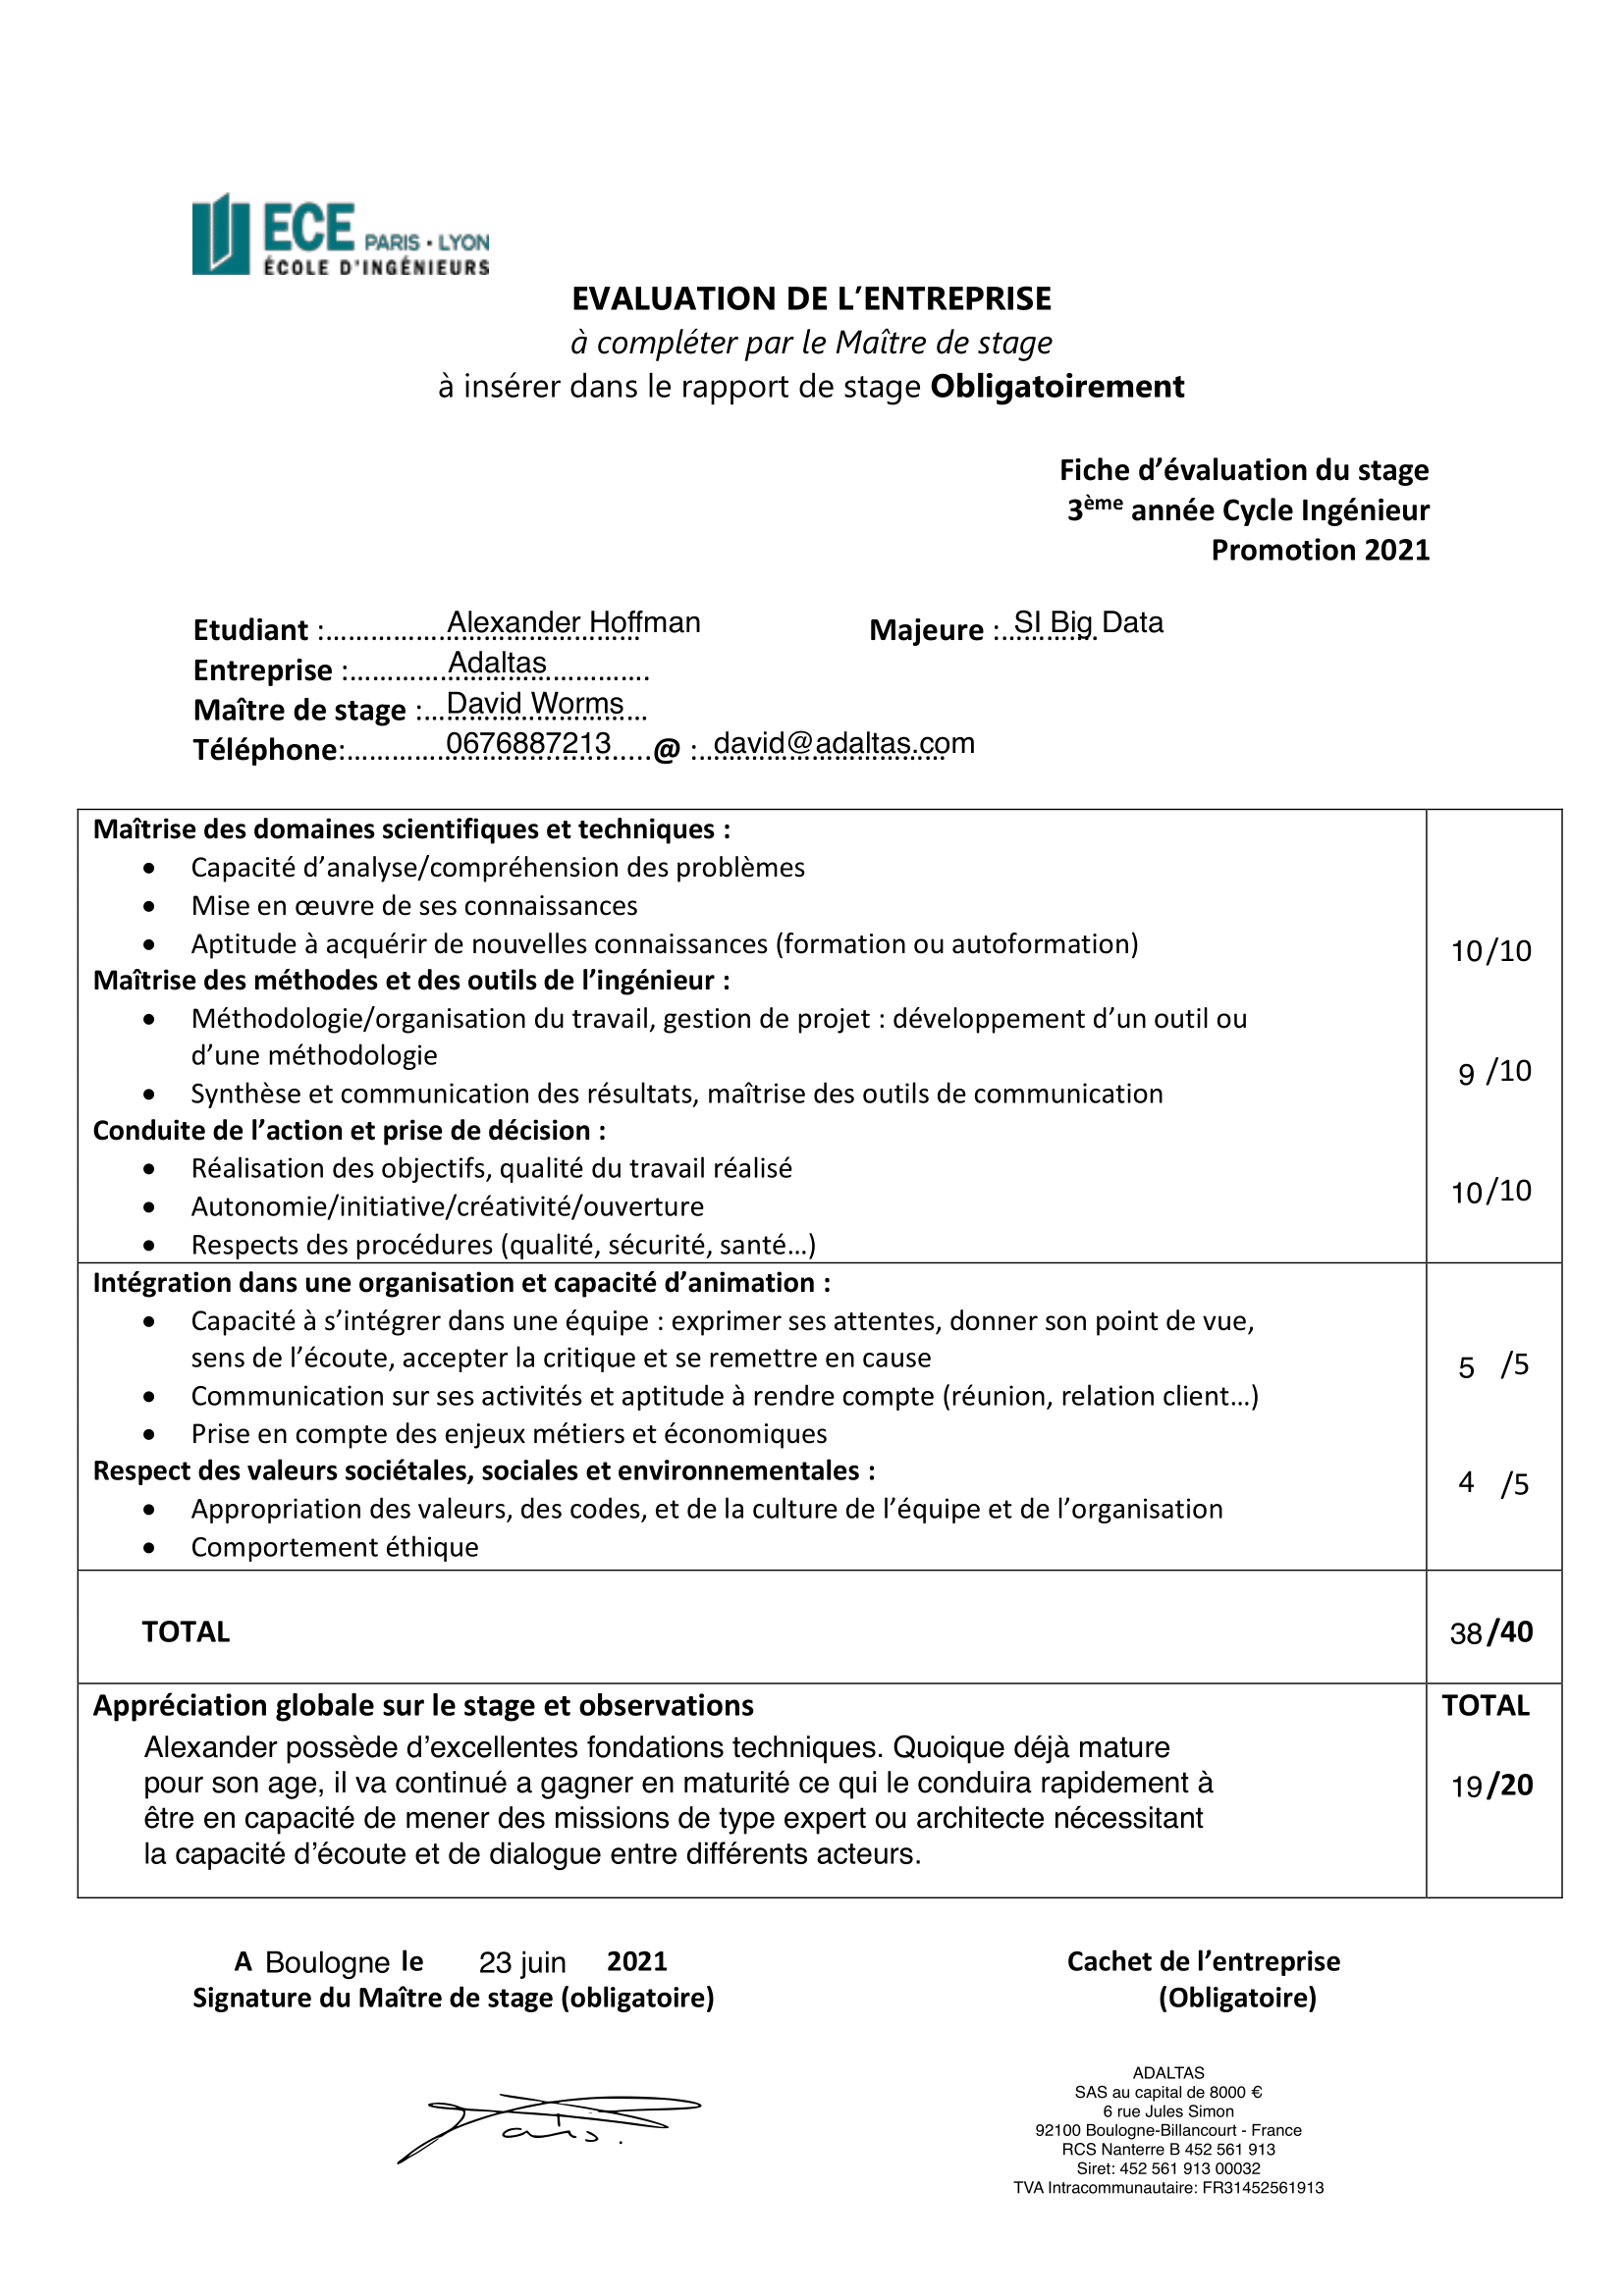
\includegraphics[scale=0.25]{assets/img/evaluation.png}
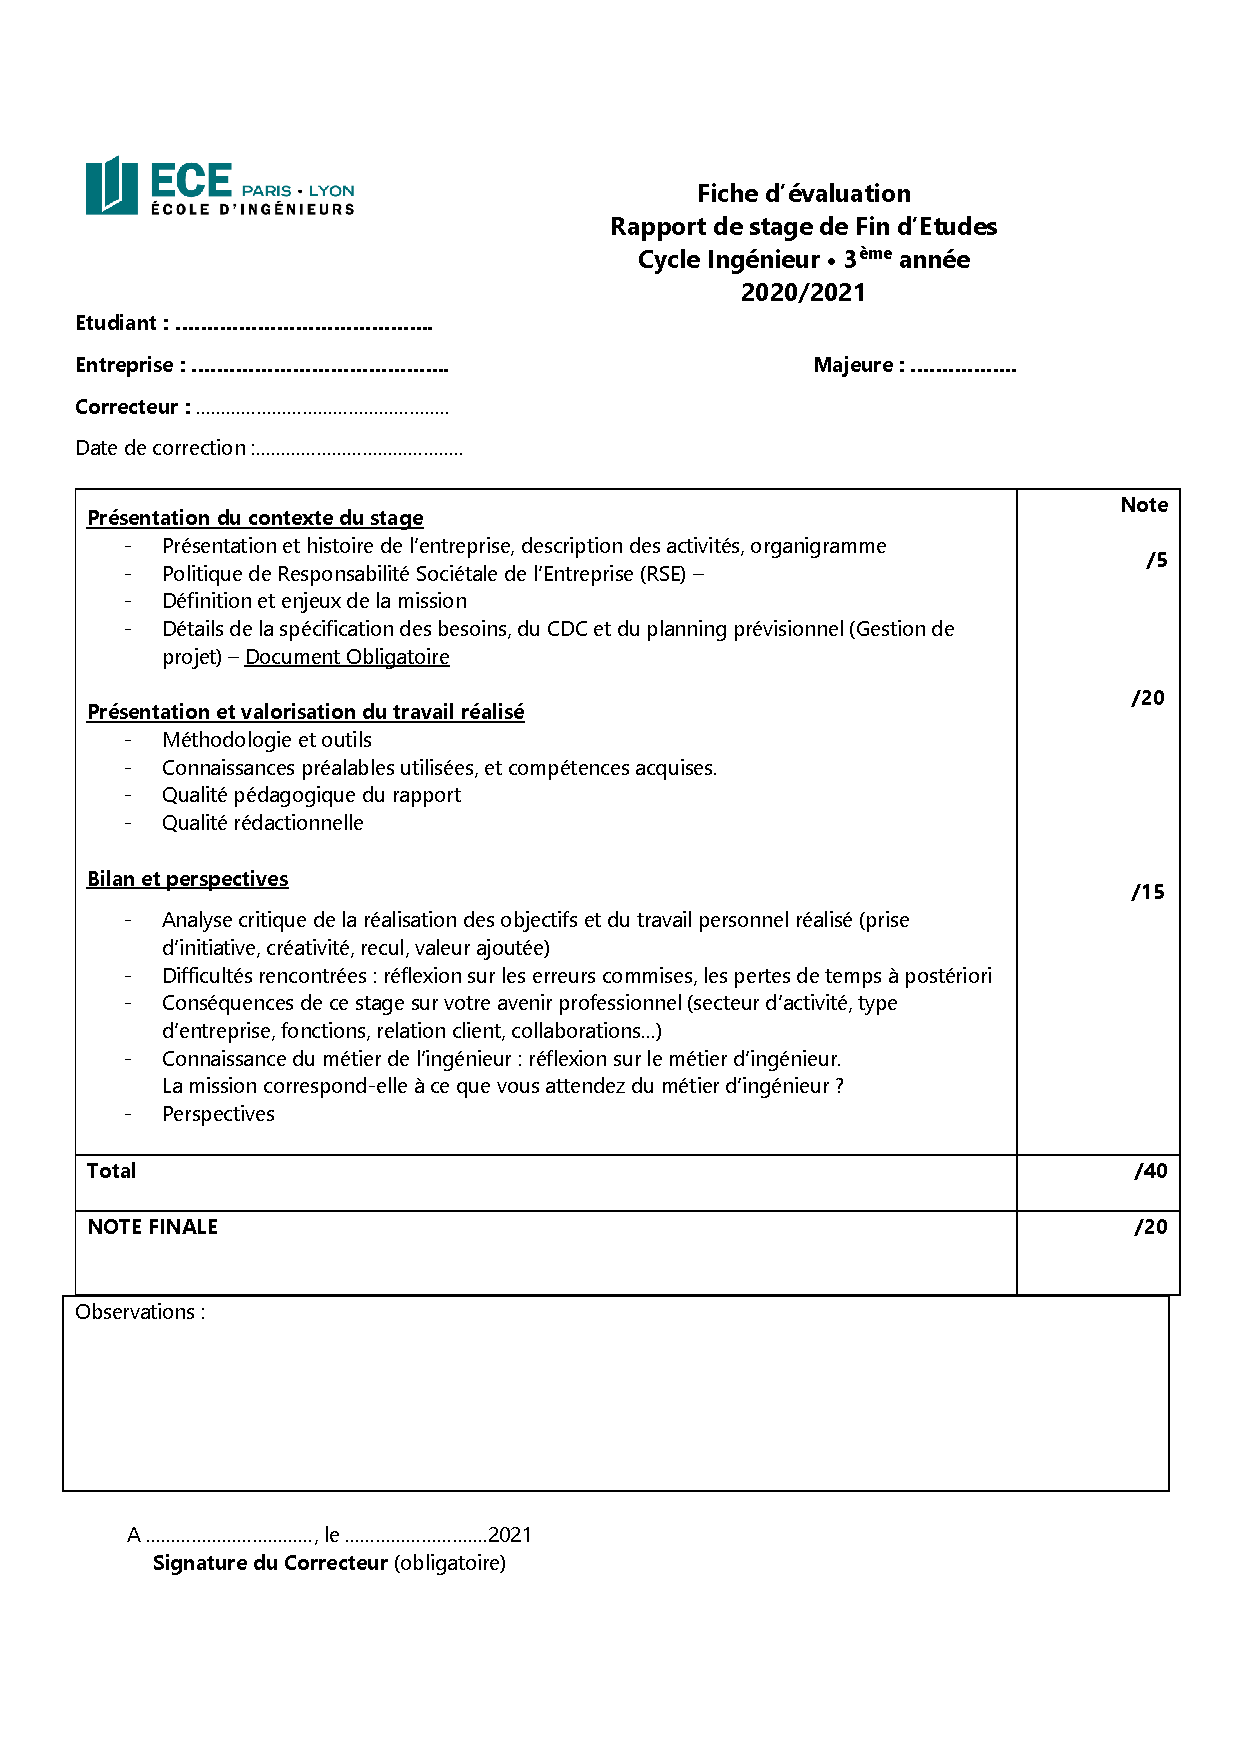
\includepdf[pages=-]{assets/pdf/eval-rds.pdf}
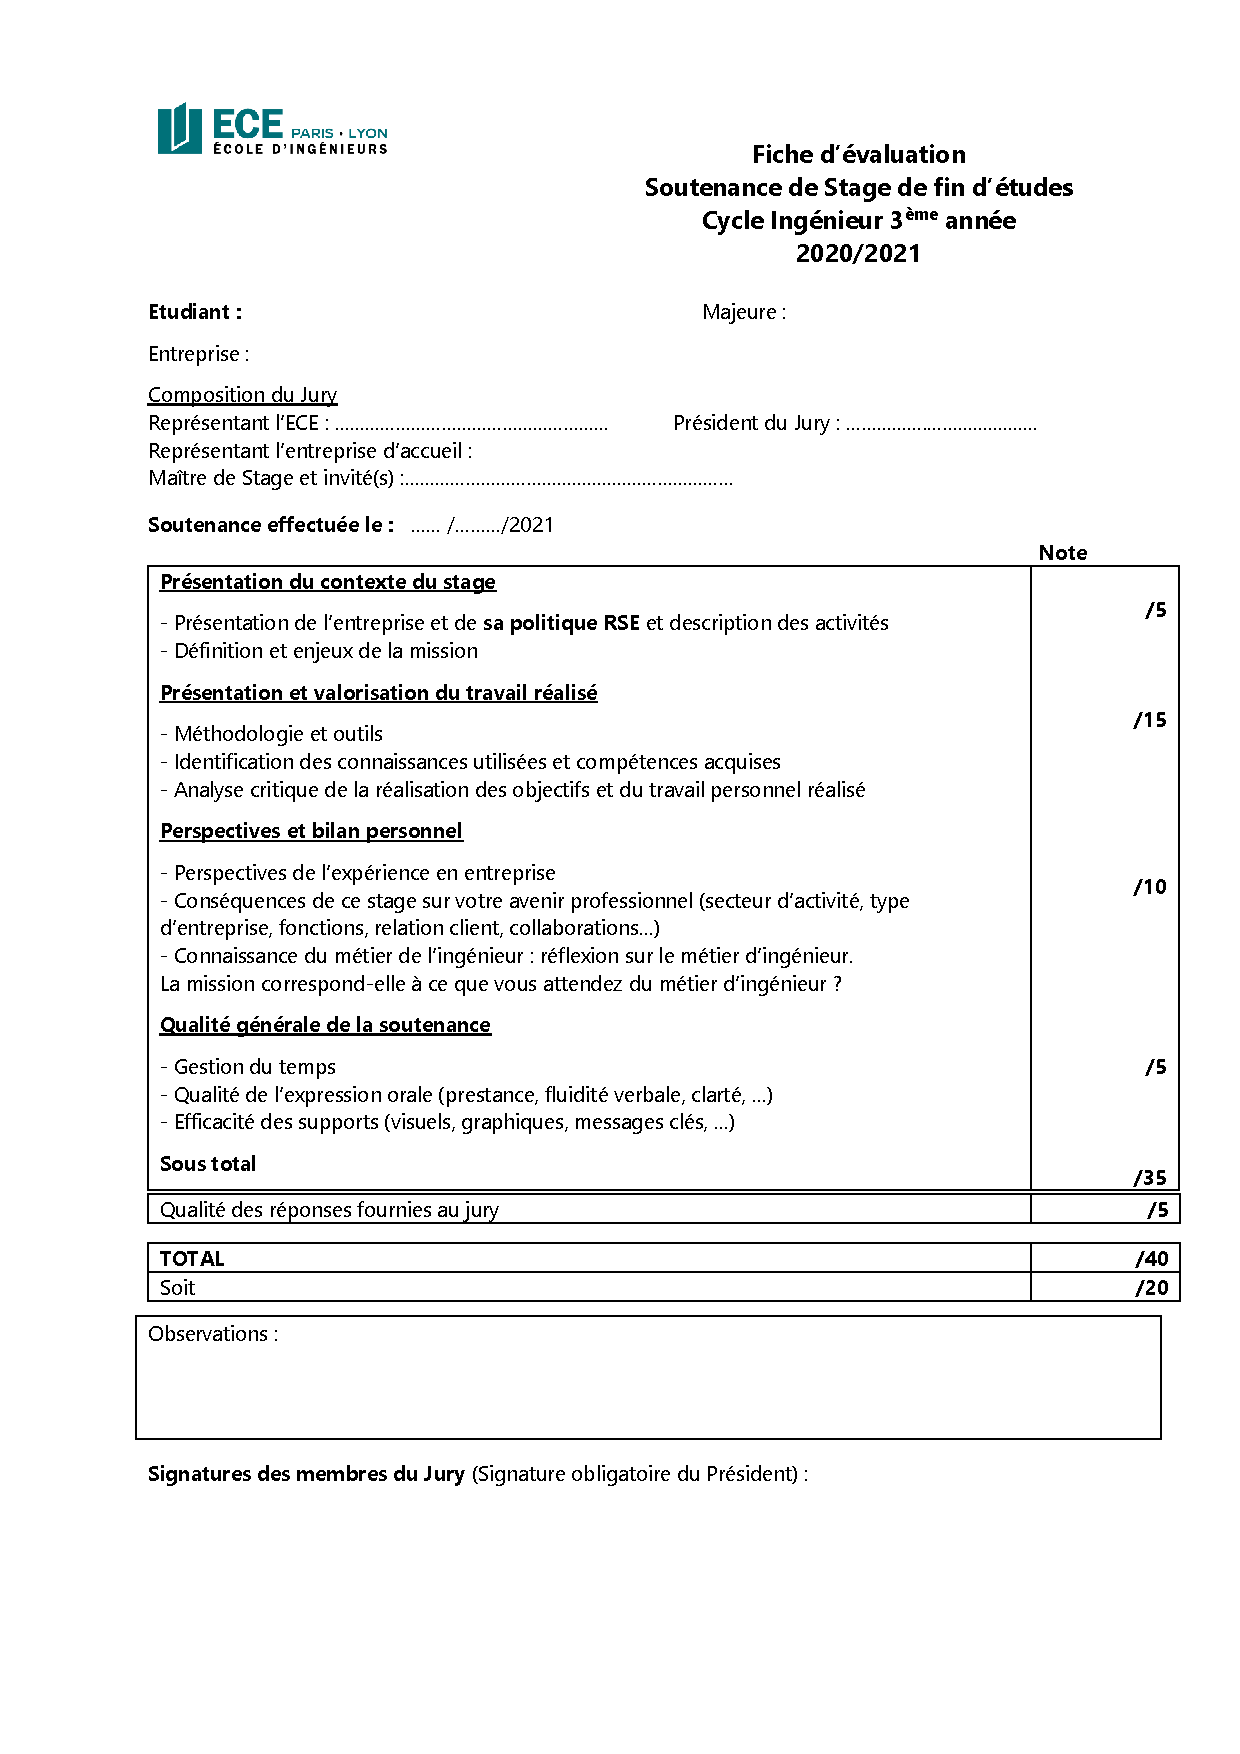
\includepdf[pages=-]{assets/pdf/eval-soutenance.pdf}

\end{document}

